%%%%%%%%%%%%%%%%%%%%%%%%%%%%%%%%%%%
\chapter{{RESULTS AND DISCUSSION}} \label{chap:4}
%%%%%%%%%%%%%%%%%%%%%%%%%%%%%%%%%%%
%%%%%%%%%%%%%%%%%%%%%%%%%%%%%%%%%%%
\section{Introduction}
%%%%%%%%%%%%%%%%%%%%%%%%%%%%%%%%%%%
In this chapter we present, discuss, and analyze the main findings of our work. Our work explains  the molecular dynamics study of transport and thermodynamic properties of methane and various gases in water at different temperatures. In the section of  transport properties,  we discuss  the diffusivity and mobility of the studied systems whereas in the section of  thermodynamic properties, we discuss the free energy of solvation of the systems in different liquid environments. The findings of the present work will cover the following topics.

\begin{enumerate}
 \item  The investigation of the diffusion of gases  in water is undertaken in order to test  out the various empirical relations  relating the diffusion coefficients to various molecular properties of the gases. This study discusses the structural and transport properties of first four light alkanes (methane, ethane, propane and n-butane) in SPC/E water. In addition to this, we discuss the diffusion of NO, Co and N2 molecules in SPC/E water at different temperatures.  
  
  \item Water is the most important fluid and a universal solvent  in nature, and aqueous electrolyte solutions  are ubiquitous components of environmental, geochemical, industrial and biological systems.  In this study, we  have calculated the diffusion coefficients  and mobilities of alkali metal cations $Na^{+}$, $K^{+}$ and halide anions $F^{-}$, $Cl^{-}$, $Br^{-}$, $I^{-}$ in  water at infinite dilution  at 25 $^{\circ}$C. 
  
  \item  Hydrophobic or amphiphilic interactions between the amino acids side-chain residues and the liquid  environment controls the motion of biological macromolecules such as protein and nucleic acids and biological processes like protein folding and their denaturation. The  present study discusses the solvation free  energy for light alkane (methane, ethane, propane and n-butane) dissolved in water and methanol  respectively over a wide range of temperatures.
\end{enumerate} 

We go through the diffusion of  gaseous methane including other three light alkanes, CO, NO, N2 in water,  diffusion coefficients  and mobilities of alkali metal cations $Na^{+}$, $K^{+}$ and halide anions $F^{-}$, $Cl^{-}$, $Br^{-}$, $I^{-}$ in water at infinite dilution and  solvation of    light alkanes (methane, ethane, propane and n-butane) dissolved in water and methanol  respectively over a broad range of temperatures in the sections~\ref{methanegas},~\ref{ions} and~\ref{solvation}, respectively.
%%%%%%%%%%%%%%%%%%%%%%%%%%%%%%%%%%%
\section{Methane and other lighter alkanes, NO, CO, and N2 in water} \label{methanegas}
%%%%%%%%%%%%%%%%%%%%%%%%%%%%%%%%%%%
Structural and transport properties of first four alkanes (methane, ethane, propane and n-butane), NO, CO, N2 in water have been calculated by using MD simulation technique at different temperatures (Section ~\ref{methane_diffusion}). In this work, we have estimated self diffusion coefficients along with the binary diffusion coefficients of mixtures of different gases in water  (studied system)  at different temperatures ranging from 283.15 K to 333.15 K. The role of interaction in the structure of the constituents of the system  as a function of temperature is studied with the help of the radial distribution function (RDF) and the coordination numbers. The self-diffusion coefficient of the solvent (water) is calculated by using mean square displacement (MSD) method  where as that for solute (gases)  is calculated by using MSD  and velocity auto correlation function (VACF) methods~\citep{Allen1989, Frenkel2002}. In the following subsections we discuss the energy profile, simulated densities and temperatures,  structural  and dynamical properties of the studied systems.
   
%%%%%%%%%%%%%%%%%%%%%%%%%%%%%%%%%%%
\subsection{Energy Profile, Density and Temperature}
%%%%%%%%%%%%%%%%%%%%%%%%%%%%%%%%%%%
In this section we discuss the energy profile of the system under study. There exists different interactions between atoms which give rise to the different energies. Energy profile portrays all such energies due to these interactions. Intra-molecular movements like bond stretches, angle vibrations, dihedral rotations contribute to energy of the system and interactions pertaining to these behaviors are
categorized as bonded interactions. Atoms of the system whether these are intra-molecular or inter-molecular interact with each other through Coulomb potential and LJ potential. These come inside non-bonded interactions. Intra-molecular non-bonded interactions comprise Coulomb-14 and LJ-14 interactions~\citep{Allen1989, Gromacs-manual}. Bonded and non-bonded interaction energies contribute to the potential energy of the system and sum of potential energy and kinetic energy finally gives the total energy of the system.

The energy minimization of the system is done to obtain the stable, low energy configuration by changing the geometry of a structure. Energy minimization is the method of identifying a point in the configuration space at which the net force on each atom vanishes. It is done before attempting MD simulation because the process of solvation of the atoms introduces some bad contacts that need to be relaxed before we give the kinetic energy. In energy minimization, the potential energy function(or force field) is evaluated by a certain algorithm or minimizer that moves the atoms nearest to a
nearest local minimum (not necessarily the global minimum). In this work,  Energy minimization is  performed   by using Steepest Descent Algorithm. Since the energy minimization changes the structure of the system from chaos to a stable structure, the local equilibrium state of the system is associated with its minimum energy after energy minimization. Figure (\ref{methane-water}) shows how the energy (potential) of the system changes in time in the course of bringing the system in a local equilibrium state. 
\begin{figure}[h!]
\centering
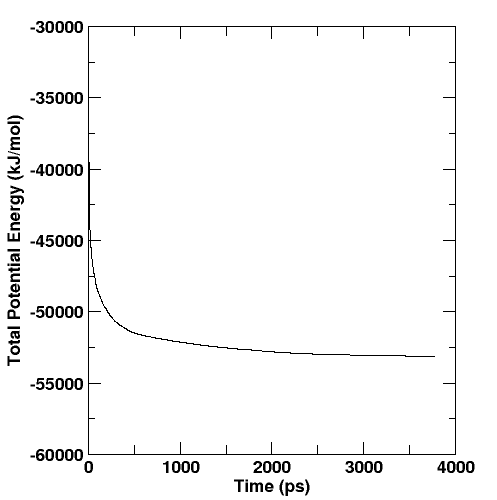
\includegraphics[width=10 cm,height= 8 cm]{Chapter4/potential.png}
\caption[Potential energy plot after Energy minimization.]{Plot of potential energy as a function of time after energy minimization for methane-water system.}
\label{methane-water}
\end{figure} 
 After energy minimization, we monitored the temperature, pressure, density, and energy (potential and kinetic) of the system for the system equilibration. 
 
 We begin with the detail energy profile of the butane-water system at 283.15 K. The angle vibration potential energy is $66.69 \pm  0.098$ kJ $mol^{-1}$ and R-B potential energy is $10.49 \pm  0.018 $ kJ $mol^{-1}$. Since the bond lengths are kept fixed during the simulation, energy contribution due  to bond stretch is absent. The Coulomb short-range energy is due to the interactions  between the atoms within the cut-off length whereas the  Coulomb reciprocal energy is due  to the implementation of PME to take into account of the long-range interactions.  The value of  Coulomb short-range potential energy is $-51543.10 \pm  1.2$ kJ $mol^{-1}$ and Coulomb  reciprocal potential energy is $-3698.34 \pm 0.026$ kJ $mol^{-1}$ . The Coulomb-14 and LJ-14 potential are  the energies  due to interactions between the atoms in a molecule separated by three successive bonds. The  Coulomb-14 energy is $0.15 \pm  0.017$ kJ $mol^{-1}$ and LJ-14  energy is $18.03 \pm 0.008$ kJ $mol^{-1}$.  The  LJ short-range potential energy is $-9040.36 \pm 0.53$ kJ $mol^{-1}$ and  kinetic energy is $6956.73 \pm 0.17$ kJ $mol^{-1}$ . The total potential energy is $-46105.70 \pm 0.78$ kJ $mol^{-1}$ and total energy is $- 39149.00 \pm 0.65$ kJ $mol^{-1}$ . These are the values averaged over all the time steps and  hence are represented by a horizontal line in the respective plots (figure \ref{energyprofile-alkane}).  Looking at the energy profile (figure \ref{energyprofile-alkane}), we can observe that the Coulomb interaction (short range and reciprocal) and LJ interaction have significant contribution to the potential  energy of the system while the bonded interaction energies and the pair potential energies (14-interactions) contribute very less to the potential energy of the system. Energies due to angle vibration, R-B dihedral, Coulomb-14 and LJ-14 interactions are very less and these values almost coincide to
  the zero: these values are negligible compared to energies due to Coulomb interaction
  and LJ interaction. Coulomb energy has very large magnitude and this leads the potential energy to have negative value.  Although kinetic energy is positive, total energy  is negative due to the large negative value of potential energy. The negative value of total energy reflects the fact that our system after the equilibration run is bound and  stable. 
 \begin{figure}[h!]
 \centering
 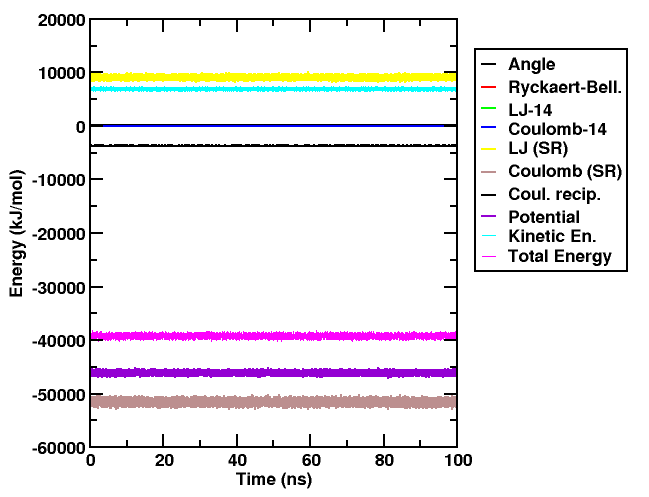
\includegraphics[width=13 cm,height= 9 cm]{Chapter4/energy_all.png}
 \caption[Energy profile of butane-water system.]{Energy profile (contribution of kinetic and potential energy) of butane-water system at  283.15 K. } 
 \label{energyprofile-alkane}
 \end{figure}
 
  We know that temperature of a particle is due to its kinetic energy. Here, we can also study the variation of kinetic energy of the system with temperature. In the table \ref{table:ke and t}, the ratios of kinetic energy to the corresponding absolute temperature are calculated and we got the same value of the ratio of kinetic energy at a temperature to the temperature and it is 24.569 kJ mol$^{-1}$ K$^{-1}$. The fifth value of constant, 24.570 kJ mol$^{-1}$ K$^{-1}$, is different from 24.569 kJ mol$^{-1}$ K$^{-1}$ but the difference is so negligible that we can conclude to have obtained the same constant value. Hence, the same constant values in the fourth column of the table \ref{table:ke and t} show that:\\
  
  $\frac{KE}{T}$ = a constant\\
  
  This means, KE  = a constant $\times$ T\\
   Or, KE is proportional to the absolute temperature.\\ 
   
   At higher temperature, molecules have higher thermal agitations and hence it affects the vibrational motion and rotational motion of atoms in the molecules. This accounts for the higher value of energies at higher temperatures  pertaining to the angle vibration and R-B dihedral.
  
 \begin{table}[H]
 \centering
 \caption[Relationship between Kinetic energy and temperature]{Relationship between Kinetic energy and temperature for butane-water system for NPT simulation}
 \label{table:ke and t}
  \resizebox{0.65\textwidth}{!}{%
   \begin{tabular}{|c|c|c|c|}
  \hline
  SN        & Temperature (T)   & Kinetic Energy (KE)  & $\frac{KE}{T}$ \\
   & in K & in kJ mol$^{-1}$ & in kJ mol$^{-1}$ K$^{-1}$\\
  \hline
  1 & 283.15 & 6956.73 & 24.569 \\
  \hline
  2 & 293.15 & 7202.50 & 24.569 \\
  \hline
  3 & 303.15 & 7447.99 & 24.569 \\
  \hline
  4 & 313.15 & 7693.67 & 24.569 \\
  \hline
  5 & 323.15 & 7939.64 & 24.570 \\
  \hline
  6 & 333.15 & 8185.09 & 24.569\\
  \hline
   \end{tabular}}
 \end{table}
 
 
 
We monitored the temperature, pressure, density, and energy of each studied system to bring it in  thermodynamic equilibrium because dynamic property like diffusion coefficient varies with
such parameters.  The density and simulated temperatures at different coupling temperatures for propane-water system are shown in table (\ref{density_box}).
\begin{table}[H]
\centering
\caption[Values of simulated temperature  and density at various coupling temperatures of propane-water system.]{Values of simulated temperature ($T_{sim}$) and density at various coupling temperatures ($T_{co}$) of propane-water system.}
\label{density_box}
\resizebox{0.95\textwidth}{!}{%
\begin{tabular}{|c| c| c| c| c|}\hline
S.N &($T_{co}$) K & ($T_{sim}$) K & $\rho_{sys}$($kg/m^3$) & $\rho_{w}$($kg/m^3$)
~\citep{Pokhrel2016, Poudyal2014}\\  \hline
1 & 283.15 & 283.144$\pm$0.005 & 993.834$\pm$0.043 & 998.19\\ \hline
2 & 293.15 & 293.152 $\pm$0.010 & 989.386$\pm$0.042 & 997.30\\ \hline
3 & 297.95 & 297.949$\pm$0.005 & 986.872$\pm$ 0.033 & - -\\ \hline
4 & 303.05 & 303.050$\pm$0.006 & 984.104$\pm$0.029 & - -\\ \hline
5 & 303.15 & 303.152$\pm$0.003 & 984.051$\pm$ 0.031 & 995.61\\ \hline
6 & 308.25 & 308.242$\pm$0.001 & 981.093$\pm$ 0.053 & - -\\  \hline
7 & 313.15 & 313.153 $\pm$0.007 & 978.44  $\pm$ 0.059 & 994.20 \\ \hline
8 & 315.75 & 315.753$\pm$0.003 &  976.435$\pm$ 0.050 & - -\\ \hline
9 & 323.15 & 323.142 $\pm$0.003 & 971.565   $\pm$0.031  & 992.17\\  \hline
10 & 333.15 & 333.152 $\pm$0.006 & 964.396 $\pm$ 0.048  & 987.99\\ 
\hline
\end{tabular}}
\end{table}
 Table (\ref{density_box}) shows that our simulated value of system density is in maximum deviation of around 1$\%$ with that of water density. 
  
  %%%%%%%%%%%%%%%%%%%%%%%%%%%%%%%%%%%
  \subsection{Structural Analysis  of the  Systems}
  %%%%%%%%%%%%%%%%%%%%%%%%%%%%%%%%%%%
  Each molecule in a liquid is in constant interaction with a large number of its  neighbors. When the terminology liquid structure is used, one is referring to
  quantities like structure factor s(q), radial distribution function g(r). The advantage of molecular simulation is that we can study g(r) or s(q)~\citep{adhikari2004}. Since both g(r) and s(q) give same information, we focus on g(r). The central idea in most theories of   liquids is the radial distribution function (RDF)~\citep{mcquarrie2000}. The detail information of   g(r) is provided in chapter \ref {chap:3}.

Radial distribution functions (RDF) were obtained from the
simulations, in order to analyse the local structure around the solute and solvent molecule.  Radial distribution function (RDF) gives the 
idea of distribution of neighboring molecules with respect to the reference molecule considered in the calculations. In periodic systems, RDF
shows sharp peaks and troughs up to infinity where the separations and heights are the characteristics of the lattice structure. In liquids however, RDF oscillates up to certain orders and then attains constant value as unity~ \citep{mcquarrie2000}.


%%%%%%%%%%%%%%%%%%
\begin{figure}[h!]
\begin{center}
\subfigure[]{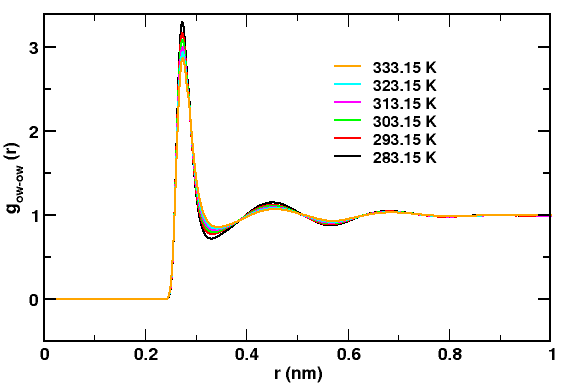
\includegraphics[height =7cm, width =7.32cm]{Chapter4/rdf_owow.png}} 
\subfigure[]{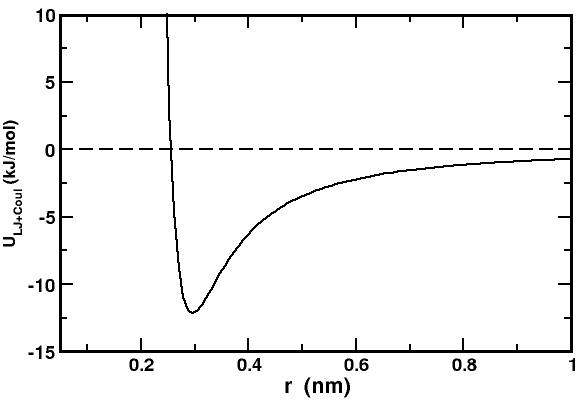
\includegraphics[height =7cm, width =7.32cm]{Chapter4/cuol.png}}
\caption[RDF of oxygen atoms of water molecules and  Lennard-Jones plus Coulomb potential for two isolated water molecules.] {(a) RDF of oxygen atoms of water molecules at different temperatures  (b)  Lennard-Jones plus Coulomb ($\mathrm{U_{LJ+Coul}}$) potential as a function of distance for two different isolated water molecules~ \citep{pokharel2018transport, Pokhrel2016}}
\label{rdfowow}
\end{center}
\end{figure}
%%%%%%%%%%%%%%%%%%

Figure \ref{rdfowow}(a) represents the RDF of oxygen atoms of water molecules at different temperatures. For the structure  of the water molecule, the centre of mass is practically the same as the oxygen centre, which is also the van de Waals sphere centre. This makes the results for the oxygen atom representative of the whole water molecule. The figure explores three different peaks which implies that the molecules are correlated up to third solvation shell. The value of $\sigma$ for OW-OW is 0.3165 nm, and the van der Waals radius (2$^{\mathrm{1/6}}\sigma$) is 0.3553 nm~ \citep{Gromacs-manual}. The figure \ref{rdfowow}(a) shows that excluded region remains fairly independent (0.276 $\pm$ 0.002 nm) of changing temperature. It also calculates that the excluded region is smaller than the van der Waals radius which indicates the contributions from other potentials in addition to the van der Waals potential~\citep{pokharel2018transport, Pokhrel2016} (see Fig.\ref{rdfowow}b). The first peak position remains at the same position within the error of $\pm$ 0.002 nm as a function of temperature. The magnitudes of all the peaks in RDFs decrease on rising temperature. Furthermore, the width of the peaks increases on increasing temperature. Both variations are the consequences of excess volume created in the system and  the  decrease in co-ordination number  with increase in temperature. These results show that the movement of the particles enhances and the solvent becomes less structured as temperature is increased. The  figures \ref{rdfowow} (a) and that  of  \ref{rdfowow} (b)~\citep{pokharel2018transport, Pokhrel2016} show that  Lennard-Jones plus Coulomb potential covers almost entire potential except many body effects. The second peak and third peak positions of the $g_{OW-OW}(r)$  are 0.450 $\pm$ 0.002 nm and 0.680 $\pm$ 0.002 nm respectively. These results are in good agreement with the available references ~\citep{head2006tetrahedral,head2002water}. From the simulations, we  found that the RDFs between oxygen atoms of water molecules in different studied system for SPC/E water system are identical in all respects. It showed that the presence of the solute molecule in an infinite dilution has a negligible effect on the global structure of the solvent.

%%%%%%%%%%%%%%%%%%
\begin{figure}[h!]
\centering
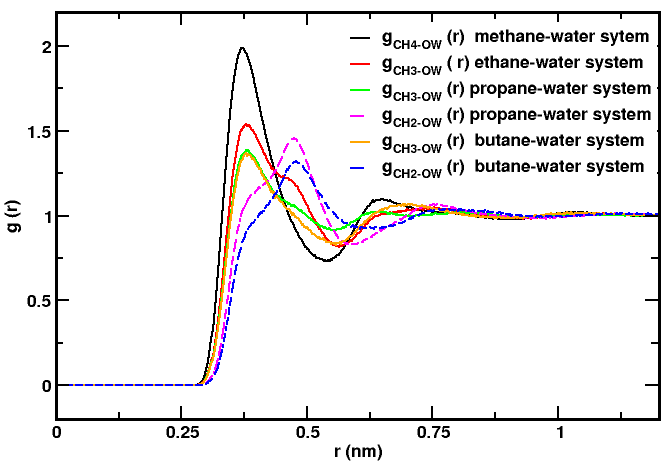
\includegraphics[height = 6.5cm]{Chapter4/rdfC-Ow.png}
\caption[Radial distribution functions between methyl and methylene carbon atoms of alkane-water system and oxygen atom of water molecule.]{Radial distribution functions between $\mathrm{CH_3}$ (solid
lines) and $\mathrm{CH_2}$ (dotted lines) and  oxygen atom of water molecule at 293.15 K.}
\label{rdfC-OW}
\end{figure}
%%%%%%%%%%%%%%%%%%

The RDF between carbon of alkane and the oxygen of water describes solute-solvent interaction. Figure (\ref{rdfC-OW}) shows the RDF between the methyl ($\mathrm{CH_3}$) and methylene ($\mathrm{CH_2}$) carbons of the alkanes and  the oxygen atom of water, calculated from the simulations at 293.15 K. In figure (\ref{rdfC-OW}), it can be seen that height of the both $\mathrm{CH_3-OW}$  and $\mathrm{CH_2-OW}$ peak clearly decrease with increase in the length  of the carbon atoms  of the alkane. The methyl carbon  groups can always approach the water molecule at closer distances (first peak position $ \sim 0.38$ nm), and the corresponding peaks are systematically more intense than the $\mathrm{CH_2-OW}$ for distances under  $\sim 0.47$ nm.  Moreover, the magnitude as well as the excluded regions for $\mathrm{g_{CH3-OW}}$ and $\mathrm{g_{CH2-OW}}$ are different. This is because methyl  and methylene carbon do not possess the same partial charge. Furthermore, when oxygen of water (OW) approaches to methyl carbon, it (or the water molecule) also experiences the interactions due to three hydrogens attached to methyl carbon and when oxygen of water (OW) approaches to methylene carbon, it (or the water molecule) experiences the interactions due two hydrogens attached to methylene carbon. This means when OW approaches to these carbons of alkane, it does not exactly experience the
same nature of interaction field around methyl and methylene carbon. 

%%%%%%%%%%%%%%%%%%
\begin{figure}[h!]
\centering
\includegraphics[height = 7.5cm]{Chapter4/{Potential_rdf.png}}
\caption[Plot of exponential of negative of interaction potential (Lennard-Jones plus Coulomb) between carbon atom of methane and water molecule and corresponding radial distribution function.]{Plot of exponential of negative of interaction potential (Lennard-Jones plus Coulomb) between carbon atom of methane and water molecule at 293.15 K. Inset: g(r) of carbon atom of methane and water molecule  at 293.15 K. }
\label{interation}
\end{figure}
%%%%%%%%%%%%%%%%%%
Fig.(\ref{interation}) represents the plot of exponential of negative of Lennard-Jones and Coulomb potential  between carbon atom of methane and water molecule as the function of  interatomic separation  and the corresponding radial distribution function at 293.15 K. The maximum of $\mathrm{exp(-\beta  U)}$ (0.31 nm) and the first peak position (FPP) of the corresponding radial distribution function (0.37 nm) are different. This shows that   Lennard-Jones plus Coulomb potential doesn't cover almost entire potential.

 Furthermore, to obtain the number of interaction sites or co-ordination number ($N_c$) of each type in a coordination shell around the reference site,  we have integrated the
radial distribution functions (RDFs) as~ \citep{mcquarrie2000}:
\begin{equation}
N_c = \int_0^{r_{min}} 4\pi~ \rho~ g(r) r^2 dr
\end{equation}
Where $\mathrm{r_{min}}$ is the radius of the coordination shell  (location of the RDF minima) and $\rho$ is the number density. We have estimated the number of sites of a given groups or molecules around another groups or molecules, as a function of the distance from its centre. 

 In figure (\ref{rdfowow}), for $g_{OW-OW}(r)$, the peak maxima ($\mathrm{r_{max}}$) of the first shell are obtained at $0.276$ nm  and the minima ($\mathrm{r_{min}}$) at $0.334$ nm for  all the alkane-water system. The first shell coordination number was found to be $5.3\pm 0.1$ for water molecules. These values or the  coordination numbers are in good agreement  with the available reference values ~\citep{head2006tetrahedral,head2002water}. The first shell   co-ordination number of water molecules around  methyl carbon is $n_H\sim 23 $, in agreement with the MAS NMR data~\citep{koh2000water}. The first cell co-ordination number  of water for  methylene carbon is greater than that of methyl carbon. Furthermore, to test the solubility of alkanes in water, we have calculated free energy of solvation of methane, ethane, propane and n-butane in water at 300 K. The estimated free energy of solvation for methane, ethane, propane and n-butane in water are $9.08 \pm 0.12$, $9.02 \pm 0.19$, $9.61 \pm 0.21$, and $10.99 \pm 0.18$ in units of $\mathrm{kJmol}^{-1}$ respectively. The values of free energy of solvation follows the same trend as reported by H. S. Ashbaugh \emph{et al.} ~\citep{ashbaugh1998hydration}. The combination of these effects; RDF analysis, co-ordination numbers of methyl and methylene carbons of alkanes and free energy of solvation of alkanes in water, suggests that the methyl groups of alkane  molecules have a preferential tendency to be dissolved in the vicinity of water molecules and that this tendency decreases with chain length. The details of the structural properties with the co-ordination numbers of water molecules around the methyl and methylene carbons of alkane-water system is provided in table \ref{coordination number}.

\begin{table}[H]
\centering
\caption[Strucural paramerters from MD simulaion of alkane-water system.]
{ Strucural paramerters from MD simulaion of alkane-water system at 293.15 K. The positions of the first maxima  ($r_{max}$), first minima ($r_{min}$), and co-ordination  numbers ($N_c$) in the first shell of the radial distribution functions are presented. } 
\label{coordination number}
\resizebox {0.55 \textwidth } {!}{%
\begin{tabular}{|c| c| c|  c| c|} \hline
system & {groups}& $r_{max}$(nm) & ~~$r_{min}$(nm) &  $N_c$
\\ \hline
CH4-H2O & CH4-water & 0.371 &  0.542  & 23.11\\ \hline  
C2H6-H2O & CH3-water & 0.378  & 0.565 & 25.49 \\ \hline 
C3H8-H2O & CH3-water & 0.381  & 0.555 & 23.18\\ \hline 
C3H8-H2O & CH2-water & 0.474  & 0.588 &28.52 \\ \hline
C4H10-H2O &  CH3-water & 0.378  & 0.558 & 22.22 \\ \hline
C4H10-H2O & CH2-water & 0.478  & 0.606 & 30.14 \\ \hline
\end{tabular}} 
\end{table} 

The RDF between the oxygen of water and oxygen of NO describes solute-solvent interaction which widens the horizon of the study, figure (\ref{rdfowon}).

%%%%%%%%%%%%%%%%%%
\begin{figure}[h!]
\centering
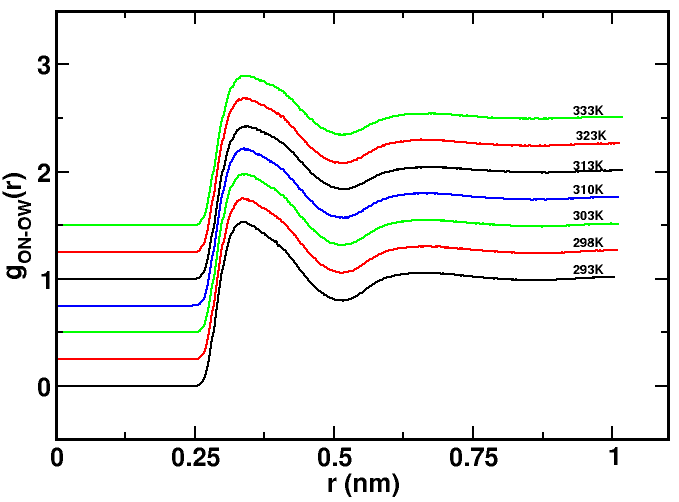
\includegraphics[height = 6.5cm]{Chapter4/g_on-ow.png}
\caption[Radial distribution function  of oxygen atom of NO molecule and oxygen atom of water molecule at different temperatures.]{Radial distribution function  of oxygen atom of NO molecule and oxygen atom of water molecule at different temperatures, from 293 K to 333 K. Along y-axis the value of g (r) is added by small amount (0.2) for each except of 293 K so that all the values are clearly seen.}
\label{rdfowon}
\end{figure}
%%%%%%%%%%%%%%%%%%

\begin{table}[H]
\centering
\caption[RDF analysis between oxygen atom of NO molecule and oxygen atom of water molecule]
{ Simulated data for the RDF analysis between oxygen atom of NO molecule and oxygen atom of water molecule at different temperatures, from 293 K to 333 K. } 
\label{rdfowontable}
\resizebox {0.55 \textwidth }{!}{%
\begin{tabular}{|c| c| c| c| c| c|} \hline
\multicolumn{6}{|c|}{RDF analysis of ON-OW}\\ \hline
T(K) & ER (nm) & FPP(nm) & FPV & SPP(nm) & SPV \\  \hline
293 & 0.258 & 0.338 & 1.536 & 0.664 & 1.058 \\ \hline
298 & 0.258 & 0.338 & 1.510 & 0.668 & 1.053 \\ \hline
303 & 0.258 & 0.343 & 1.477 & 0.676 & 1.052 \\  \hline
310 & 0.258 & 0.342 & 1.465 & 0.670 & 1.051 \\ \hline
313 & 0.256 & 0.346 & 1.425 & 0.674 & 1.043 \\ \hline
323 & 0.258 & 0.340 & 1.441 & 0.676 & 1.047 \\ \hline
333 & 0.256 & 0.340 & 1.400 & 0.678 & 1.043 \\ 
\hline
\end{tabular}}
\end{table}

 The detail of the figure (\ref{rdfowon}) is given  in table (\ref{rdfowontable}). We have observed only two peaks in radial distribution function between the solute and solvent. The magnitudes on table (\ref{rdfowontable}) shows that the excluded region remains almost fixed (with in the error of $\pm$0.004 nm) with varying temperature. The both the peak positions, FPP and SPP, shift slightly right
on elevating temperature. The peak values on the other hands decrease on rising temperature. It again signifies that correlation between NO and water decreases on increasing temperature. The value of $\sigma$ for ON-OW is 0.30895 nm, and the van der Waals
radius (2$^{\mathrm{1/6}}\sigma$) is 0.34678 nm ~\citep{zhou2005molecular, Gromacs-manual}. It shows that the van der Waals radius is greater than both the FPP (0.338 nm) and excluded region (0.256 nm).

\begin{figure}[h!]
\centering
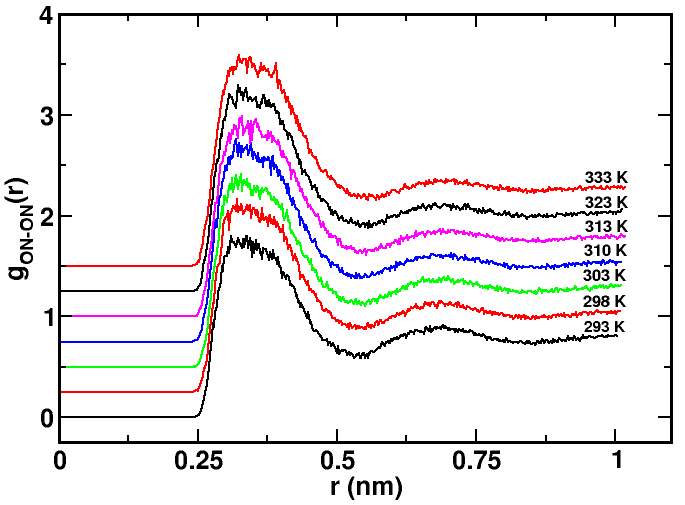
\includegraphics[height = 6.5cm]{Chapter4/g_on-on.png}
\caption[RDF between oxygen atoms of NO molecule at different temperatures]{RDF between oxygen atoms of NO molecule at different temperatures from 293 K to 333 K. Along y-axis the value of g (r) is added by small amount (0.2) for each except of  293 K so that all the values are clearly seen.}
\label{rdfonon}
\end{figure}

\begin{table}[H]
\centering
\caption[RDF analysis between oxygen atoms of NO molecule.]
{ Simulated data for the RDF analysis between oxygen atoms of NO molecule at different temperatures, from 293 K to 333 K. } 
\label{rdfonontable}
\resizebox {0.55\textwidth }{!}{%
\begin{tabular}{|c| c| c | c | c | c |} \hline
\multicolumn{6}{|c|}{RDF analysis of ON-ON}\\   \hline 
T(K) & ER (nm) & FPP(nm)& FPV & SPP(nm) & SPV \\ \hline
293 & 0.248 & 0.312 & 1.796 & 0.668 & 0.930 \\ \hline
298 & 0.246 & 0.318 & 1.914 & 0.684 & 0.908 \\  \hline   
303 & 0.246 & 0.318 & 1.909 & 0.701 & 0.894 \\ \hline
310 & 0.246 & 0.318 & 2.009 & 0.706 & 0.871\\  \hline    
313 & 0.248 & 0.330 & 1.986 & 0.686 & 0.869 \\ \hline
323 & 0.246 & 0.322 & 2.051 & 0.676 & 0.871 \\ \hline
333 & 0.244 & 0.324 & 2.090 & 0.675 & 0.865 \\ \hline
\end{tabular}}
\end{table}
 Figure (\ref{rdfonon}) represents the RDF of oxygen atoms of NO molecules. The details of the figure (\ref{rdfonon}) is given in table (\ref {rdfonontable}). The value of $\sigma_{ON-ON}$ is 0.2875 nm and the value of van der Waals radius is 0.32271 nm. The excluded region is less than van der Waals radius and first peak position is nearly equal to van der Waals radius. The roughness in the
figure (\ref{rdfonon})  is due to the less statistics (only 5 NO molecules).

We then study the RDF between oxygen atom of CO molecule and oxygen atom of water molecule
which is shown in figure (\ref {rdfocow}).
\begin{figure}[h!]
\centering
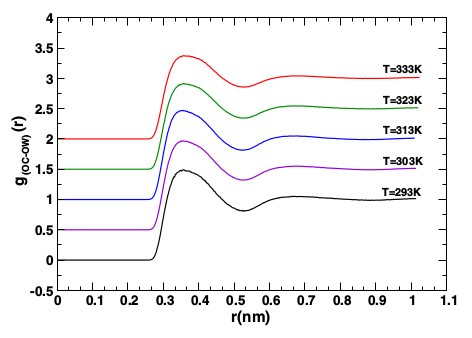
\includegraphics[height = 6.5cm]{Chapter4/rdf_ocow.png}
\caption[Radial distribution function  of oxygen atom of CO molecule and oxygen atom of water molecule at different temperatures.]{Radial distribution function  of oxygen atom of CO molecule and oxygen atom of water molecule at different temperatures, from 293 K to 333 K. Along y-axis the value of g (r) is added by small amount (0.5) for each  except of  293 K  so that all the values are clearly seen.}
\label{rdfocow}
\end{figure}

From figure (\ref{rdfocow}) one can see two different peaks and the value of the peak and
position of the peak in detail is provided in table (\ref {rdfocowtable}). 

\begin{table}[H]
\centering
\caption[RDF analysis between oxygen atom of CO molecule and oxygen atom of water molecule]
{ Simulated data for the RDF analysis between oxygen atom of CO molecule and oxygen atom of water molecule at different temperatures, from 293 K to 333 K. } 
\label{rdfocowtable}
\resizebox {0.55 \textwidth }{!}{%
\begin{tabular}{|c |c |c| c| c| c|} \hline
\multicolumn{6}{|c|}{RDF analysis of OC-OW}\\ \hline
T(K) & ER (nm) & FPP(nm) & FPV & SPP(nm) & SPV \\ \hline
293 & 0.252 & 0.356 & 1.491 & 0.668 & 1.054 \\ \hline
303 & 0.248 & 0.356 & 1.470 & 0.676 & 1.053 \\ \hline
313 & 0.250 & 0.354 & 1.471 & 0.676 & 1.050 \\ \hline
323 & 0.246 & 0.356 & 1.416 & 0.674 & 1.047 \\ \hline
333 & 0.248 & 0.356 & 1.375 & 0.668 & 1.044 \\ \hline
\end{tabular}}
\end{table}

The positions of the first peak and second peak doesn't follow a trend. The value
of first peak and second peak decreases slightly with the increase in temperature.
This signifies that the correlation between carbon monoxide and water molecules
decreases with the rise in temperature which is caused by the increased thermal
energy acquired by the molecules. The value of $\sigma_{oc-ow}$  is 0.315 nm and the van
der Waals radius is 0.354 nm. It is seen from table (\ref {rdfocowtable}) that the value of first
peak point is greater than van der Waals radius and the excluded region is less
than the van der Waals radius of oxygen atoms of two different types of molecule
of the system.


Figure (\ref{rdfococ}) shows the RDF of oxygen atoms of carbon monoxide molecule.
\begin{figure}[h!]
\centering
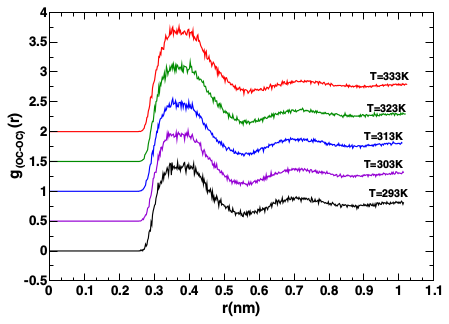
\includegraphics[height = 6.5cm]{Chapter4/rdf_ococ.png}
\caption[RDF between oxygen atoms of CO molecule at different temperatures]{RDF between oxygen atoms of CO molecule at different temperatures from 293 K to 333 K. Along y-axis the value of g (r) is added by small amount (0.5) for each except of  293 K so that all the values are clearly seen.}
\label{rdfococ}
\end{figure}
From figure (\ref{rdfococ}) one can see two different peaks and the value of the peak and
position of the peak in detail is provided in table (\ref {rdfococtable}).

\begin{table}[H]
\centering
\caption[RDF analysis between oxygen atoms of CO molecule.]
{ Simulated data for the RDF analysis between oxygen atoms of CO molecule at different temperatures, from 293 K to 333 K. } 
\label{rdfococtable}
\resizebox {0.55\textwidth }{!}{%
\begin{tabular}{|c| c| c |c| c |c|} \hline
\multicolumn{6}{|c|}{RDF analysis of OC-OC}\\   \hline 
T(K) & ER (nm) & FPP(nm)& FPV & SPP(nm) & SPV \\  \hline
293 & 0.258 & 0.366 & 1.487 & 0.706 & 0.908 \\ \hline
303 & 0.254 & 0.368 & 1.488 & 0.694 & 0.880 \\ \hline
313 & 0.254 & 0.352 & 1.553 & 0.690 & 0.894 \\ \hline 
323 & 0.256 & 0.354 & 1.632 & 0.718 & 0.875 \\  \hline
333 & 0.252 & 0.352 & 1.752 & 0.720 & 0.860 \\ \hline
\end{tabular}}
\end{table}

The value of $\sigma_{oc-ow}$ is 0.310 nm and the value of van der Waals radius is 0.351 nm.
The excluded region is less than van der Waals radius and first peak position is greater than van der Waals radius. The nature of the rough peak, clearly visible in the figure (\ref{rdfococ}), is due to the lesser number of carbon monoxide molecule. This in turn plays a role for undefined trend in the position and values of the peaks, as temperature increases. Although our simulated system contains only 5 carbon
monoxide (CO) molecules and 280 water molecules, the RDF we have calculated informs that these CO molecules do not move independently of each other and are, therefore, correlated to some extent, ascertaining that the system cannot be considered to be perfectly infinitely dilute.

%%%%%%%%%%%%%%%%%%
\begin{figure}[h!]
\centering
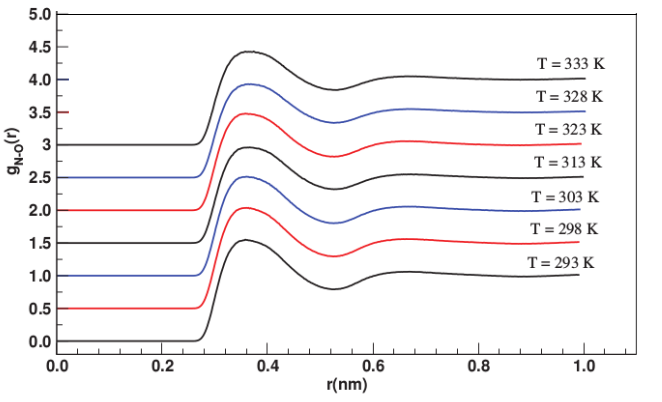
\includegraphics[height = 6.5cm]{Chapter4/rdf_no.png}
\caption[Radial distribution function  of nitrogen atom of N2 molecule and oxygen atom of water molecule at different temperatures.]{ Radial distribution function  of nitrogen atom of N2 molecule and oxygen atom of water molecule, $g_{N-O} (r)$ at different temperatures, from 293 K to 333 K. Along y-axis the value of g (r) is added by small amount (0.5) for each  except of  293 K  so that all the values are clearly seen.}
\label{rdfno}
\end{figure}
%%%%%%%%%%%%%%%%%%

Figure (\ref {rdfno}) is a plot of radial distribution function, $g_{N-O} (r)$, as a function of separation distance for the nitrogen atom of nitrogen molecules and oxygen atom of  solvent molecules (water) at different temperatures. The excluded regions remain confined within 0.246 nm to 0.250 nm which is less than the van der Waal's radius 0.362 nm as expected. The position of the first and second peaks do not follow any trend. With the rise in the temperature the height of the first peaks decrease with small amount with T = 323 K as exception. Moreover, the width of the peaks increase with
the increase in temperature. This signifies that the correlation between the nitrogen and solvent molecules decreases as temperature is increased which is due to thermal energy
acquired by them as it is proportional to temperature. Table (\ref {rdfnotable}) gives the details of the radial distribution function of solvent molecules with respect to nitrogen molecules.

\begin{table}[H]
\centering
\caption[ Details of the radial distribution function between nitrogen atom of nitrogen molecule and oxygen atom of water molecule.]
{ Details of the radial distribution function between nitrogen atom of nitrogen molecule and oxygen atom of water $g_{N-O} (r)$,   at different temperatures, from 293 K to 333 K. } 
\label{rdfnotable}
\resizebox {0.55 \textwidth }{!}{%
\begin{tabular}{|c| c| c| c| c |c|} \hline
\multicolumn{6}{|c|}{RDF analysis of N-OW}\\ \hline
T(K) & ER (nm) & FPP(nm) & FPV & SPP(nm) & SPV \\ \hline 
293 & 0.248 & 0.358 & 1.552 & 0.670 & 1.062 \\ \hline
298 & 0.250 & 0.364 & 1.538 & 0.664 & 1.061 \\ \hline
303 & 0.248 & 0.360 & 1.515 & 0.674 & 1.056 \\ \hline
313 & 0.246 & 0.366 & 1.462 & 0.672 & 1.052 \\ \hline
323 & 0.248 & 0.358 & 1.479 & 0.676 & 1.057 \\ \hline
328 & 0.248 & 0.364 & 1.429 & 0.666 & 1.048 \\ \hline
333 & 0.248 & 0.374 & 1.428 & 0.682 & 1.048 \\ 
\hline
\end{tabular}}
\end{table}

%%%%%%%%%%%%%%%%%%
\begin{figure}[h!]
\centering
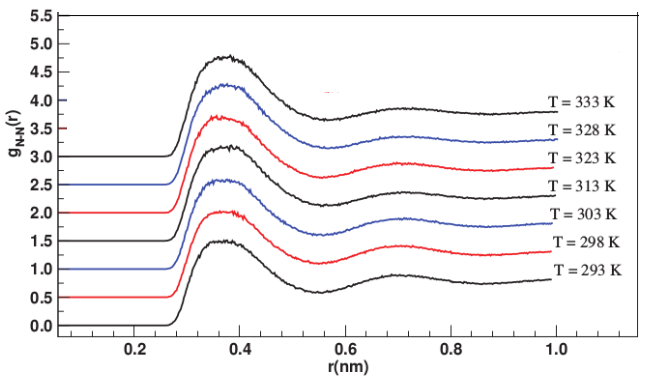
\includegraphics[height = 6.5cm]{Chapter4/rdf_nn.png}
\caption[Radial distribution function  of nitrogen atoms of N2 molecule  at different temperatures.]{ Radial distribution function  of nitrogen atoms of N2 molecule, $g_{N-N} (r)$ at different temperatures, from 293 K to 333 K. Along y-axis the value of g (r) is added by small amount (0.5) for each  except of  293 K  so that all the values are clearly seen.}
\label{rdfnn}
\end{figure}
%%%%%%%%%%%%%%%%%%

Figure (\ref {rdfnn}) gives the comparative behavior of radial distribution function of the nitrogen
atoms of N2 molecule, $g_{N-N} (r)$, as a function of separation distance at different temperatures. 
The details of the figure have been presented in table (\ref{rdfnntable}). In the
figure, it is seen that the excluded region for all temperatures remains extended to more or
less about 0.254 nm which is less than the van der Waals radius of the nitrogen molecule
0.369 nm. The position of the first peak for all temperature is more or less about 0.376
nm. Also the height of the first peak increases with increase in temperature. Moreover,
the widths of the first and second peaks increases with increase in temperature. The
height of the second peak decreases on going to higher temperature. The decrease in the
second peak and increase in width of the peaks signifies that as the temperature is raised,
the nitrogen molecules get more scattered becoming less structured.

\begin{table}[H]
\centering
\caption[ Details of the radial distribution function between nitrogen atoms of nitrogen molecule.]
{ Details of the radial distribution function between nitrogen atoms of nitrogen molecule  $g_{N-N} (r)$,   at different temperatures, from 293 K to 333 K. } 
\label{rdfnntable}
\resizebox {0.55 \textwidth }{!}{%
\begin{tabular}{|c| c| c |c| c| c|} \hline
\multicolumn{6}{|c|}{RDF analysis of N-N}\\ \hline
T(K) & ER (nm) & FPP(nm) & FPV & SPP(nm) & SPV \\ \hline 
293 & 0.254 & 0.376 & 1.512 & 0.688 & 0.905 \\ \hline
298 & 0.254 & 0.362 & 1.528 & 0.696 & 0.917 \\  \hline
303 & 0.254 & 0.376 & 1.592 & 0.712 & 0.906 \\ \hline
313 & 0.246 & 0.384 & 1.697 & 0.708 & 0.870 \\ \hline
323 & 0.254 & 0.356 & 1.720 & 0.698 & 0.870 \\ \hline
328 & 0.248 & 0.376 & 1.786 & 0.728 & 0.859 \\  \hline
333 & 0.254 & 0.382 & 1.793 & 0.728 & 0.842 \\ 
\hline
\end{tabular}}
\end{table}
 
%%%%%%%%%%%%%%%%%%%%%%%%%%%%%%%%%%%
\subsection{Diffusion Coefficients of the constituents of the System }
%%%%%%%%%%%%%%%%%%%%%%%%%%%%%%%%%%%

In this section, we discuss the self-diffusion coefficient of each component present in the systems under study. Our system is composed of water (as a solvent) and light alkanes (methane, ethane, propane and n-butane), NO, CO, N2 as solutes. We use the values of self-diffusion coefficient of each component
to determine the mutual diffusion coefficient using Darken's relation (equation \ref{darken}).

The self-diffusion coefficient of alkane (methane, ethane, propane, butane) and water are calculated by using Einstein's relation (MSD method) (equation \ref{Einstein}).

%%%%%%%%%%%%%%%%%%
\begin{figure}[h!]
\centering
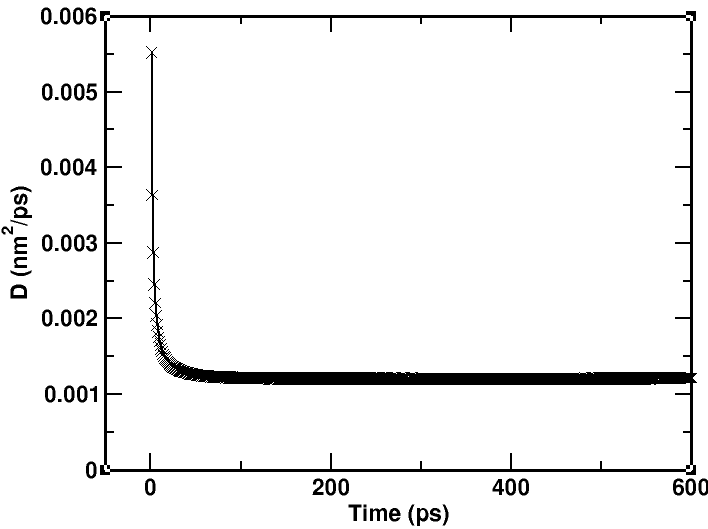
\includegraphics[height = 7.0 cm]{Chapter4/Diffusion_ethane.png}
\caption[Plot of Diffusion coefficient vs time of ethane at 283.15 K.]{Plot of Diffusion coefficient (D) = $\left\langle r^2(t)\right\rangle / 6\;t$ vs time of ethane at 283.15 K. }
\label{diffusionvstime}
\end{figure}
%%%%%%%%%%%%%%%%%%


 The figure (\ref{diffusionvstime}) shows the variation of diffusion coefficient (D) = $\left\langle r^2(t)\right\rangle / 6*t$  with time for ethane at temperature T =283.15 K. In figure (\ref{diffusionvstime}),  at first the diffusion coefficient is high due to ballistic motion and later as time passes it remains constant after 2 ns. This constant portion of the graph gives the diffusion coefficient~ \citep{Pokhrel2016}.
 
 \begin{table}[H]
  \centering
  \caption[ Self-diffusion coefficients of water at different temperatures.]{Self-diffusion coefficients of water at different temperatures and the reference experimental values.} 
  \label{water_diffusion}
 \resizebox {0.60 \textwidth } {!}{%
  \begin{tabular}{| c| c | c| } \hline
 \multicolumn{3}{|c|}{Diffusion Coefficient ( $\times$10$^{-\mathrm{9}}$ m$^\mathrm{2}$s$^{-\mathrm{1}}$)} \\ \hline 
 Temperature (K) &  Simulated Value   &  Experimental Value ~\citep{easteal1989diaphragm} \\ \hline
 283.15 & $1.71\pm 0.009$ & 1.54  \\ \hline  
 293.15 & $2.18 \pm 0.006$ & 2.02    \\   \hline
 297.95 & $2.43\pm 0.036$ & -- \\   \hline
 303.05 & $ 2.70\pm 0.008$ & --   \\ \hline
 303.15 &  $ 2.73\pm 0.005$ & 2.59    \\ \hline
 308.25 &  $ 3.01\pm 0.040$ & --   \\ \hline
 313.15 &   $ 3.30\pm 0.080$ & 3.24    \\  \hline
 315.75 &   $ 3.46\pm 0.092$ & --   \\ \hline
 323.15 &  $ 3.95\pm 0.085$ & 3.96   \\ \hline
 333.15 & $ 4.64\pm 0.120$ & 4.77    \\ \hline
 \end{tabular}} 
 \end{table}  
 
 Figure (\ref{msdalkanewater})  show the MSD plot of alkane  and water at different temperatures respectively. The value of self-diffusion coefficients of the desired species is calculated using equation (\ref{Einstein}).  In our case, we have a simulation time of 100 ns and the best statistics for alkane (methane, ethane, propane and n-butane) molecule is found within 2 ns which can also be justifiable from figure (\ref{diffusionvstime}) and is very small in comparison to simulation time; this is due to lesser number of alkane molecules. For water molecule best statistics is found within 5 ns due to larger number of water molecules. The binary diffusion coefficient of the alkane-water system is estimated using Darken's relation (Equation (\ref{darken})). Our system consists of 3 alkane molecules (methane, ethane, propane and n-butane each)  and 971 water molecules, a separate sytem, so the mole fraction for alkane is 0.003 and that of water is water is 0.997. The binary diffusion coefficient is  very close to that of self-diffusion coefficient of solute in the mixture due to low solute concentrations studied in this work.
 
  
 %%%%%%%%%%%%%%%%%%
 \begin{figure}[h!]
 \begin{center}
 \subfigure[]{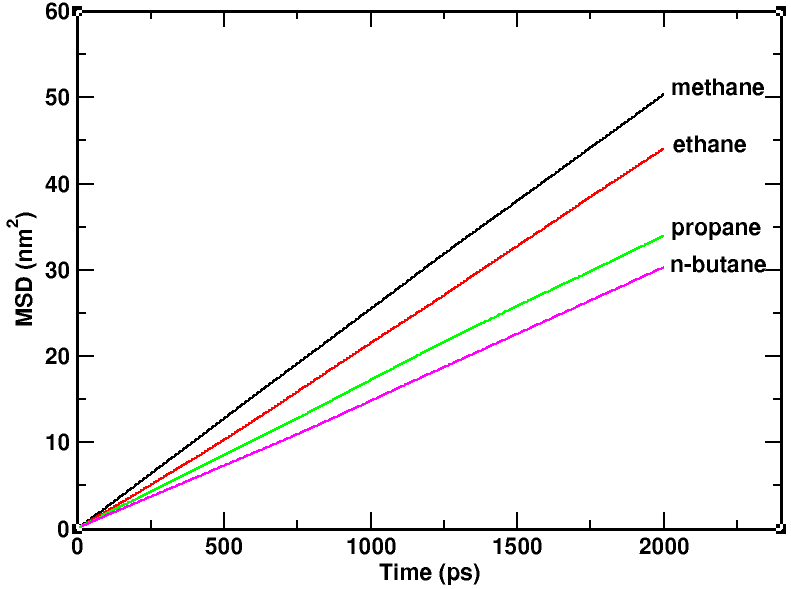
\includegraphics[height =7cm, width =7.32cm]{Chapter4/msd_alkane.png}} 
 \subfigure[]{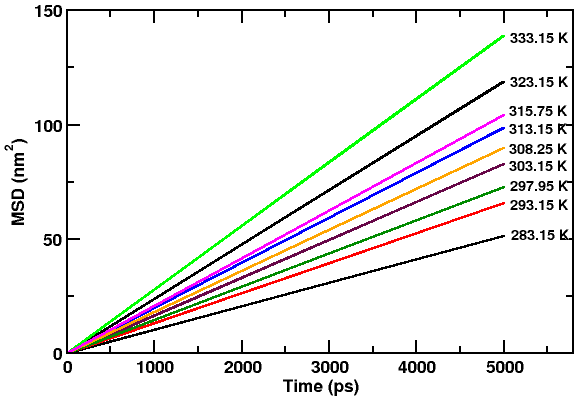
\includegraphics[height =7cm, width =7.32cm]{Chapter4/msd_h20_all.png}}
 \caption[Plot of mean square displacement (MSD) vs time of alkanes (methane, ethane, propane, n-butane) and water.] {(a) Plot of mean square displacement (MSD) vs time of alkanes (methane, ethane, propane, n-butane) in water at temperature 333.15 K. (b) Plot of MSD vs time of water at different temperatures.}
 \label{msdalkanewater}
 \end{center}
 \end{figure}
 %%%%%%%%%%%%%%%%%%
 
  Figure (\ref{carbon}) shows the variation of binary diffusion coefficients of the molecule with increasing the numbers of carbon atoms of the alkane chain. The diffusion coefficents of the molecules decreases with increasing the number of carbons present in the alkane molecules. Thus, the diffusion coefficients of methane is highest and that of n-butane is lowest among the studied system.

 %%%%%%%%%%%%%%%%%%
 \begin{figure}[h!]
 \centering
 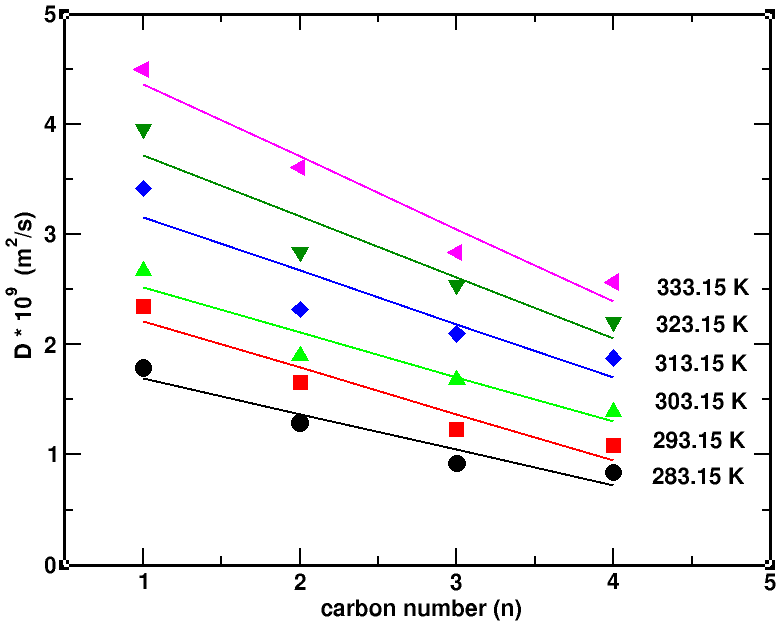
\includegraphics[height = 7.5 cm]{Chapter4/diffusion_carbon.png}
 \caption[The variation of simulated values of binary diffusion coefficients  of alkanes in water  with the numbers of carbon atoms.] {The variation of simulated values of binary diffusion coefficients  of alkanes in water  with the numbers of carbon atoms in the alkane chain  at different temperatures } 
\label{carbon}
\end{figure}
 %%%%%%%%%%%%%%%%%%
 
 %%%%%%%%%%%%%%%%%% 
\begin{figure}[h!]
 \centering
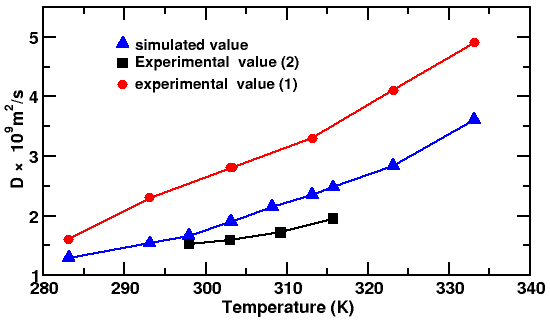
\includegraphics[height = 7.5 cm]{Chapter4/ethane_diffusion.png}
\caption[Comparison of simulated and experimental values of binary diffusion coefficients of ethane-water system.]{ Comparison of simulated and experimental values of binary diffusion coefficients of ethane-water system at different temperatures.}
\label{compare}
\end{figure}
 %%%%%%%%%%%%%%%%%%
 
 The values of self diffusion coefficients of water ($\mathrm{H_2O}$)  and binary diffusion coefficients of alkane (methane, ethane, propane, n-butane) in water   along with the references at different temperatures are presented in table  (\ref{water_diffusion}) and table (\ref{diffusion_table}) respectively . The comparison of the values from the tables and also from other references explores that self-diffusion coefficients of water from the present work, in general, come in very good agreement with the previous studies ~\citep{Pokhrel2016, Thapa2013, Poudyal2014, easteal1989diaphragm}. The experimental and simulated values of self-diffusion coefficients of water in all system are in good agreement with maximum  deviation of $11\%$  at 283.15 K ~\citep{easteal1989diaphragm}. 
  \begin{table}[H]
  \centering
  \caption[The simulated value of binary diffusion coefficient of alkanes (methane, ethane, propane, n-butane) and also the references for them as a function of temperature are listed.]{The simulated value of binary diffusion coefficient of alkanes (methane, ethane, propane, n-butane)  and also the references for them as a function of temperature are listed.}
 \label{diffusion_table}
 \resizebox {1.00 \textwidth }{!}{%
 \begin{tabular}{|c| c| c| c| c| }
 \hline 
 \multicolumn{5}{|c|}{Diffusion Coefficient ( $\times$10$^{-\mathrm{9}}$ m$^\mathrm{2}$s$^{-\mathrm{1}}$)} \\  
 \hline   System & Temp.(K) & Simulation & Expt.(1)~\citep{wise1966diffusion} &  Expt.(2)~\citep{witherspoon1965diffusion}, Expt.(3)~\citep{witherspoon1969correlation}  \\ \hline
  &  283.15 &  $1.79 \pm 0.10$ & 1.9 & ---    \\
  & 293.15 &  $2.08 \pm 0.08$ & 2.4 & $1.49 \pm 0.04$ (3) \\
  & 297.95 &  $2.35 \pm 0.08$ & --- & $1.88 \pm 0.01$ (2)   \\
  & 303.05 &  $2.56 \pm 0.12 $ & --- & ---   \\
 CH4-H20 & 303.15 & $2.60 \pm 0.06$ & 3.0 & --- \\
  & 308.25 & $2.80 \pm 0.11$ & --- &  $2.12 \pm 0.03$ (2)   \\
  & 313.15 &  $3.34 \pm 0.10$& 4.2 & $2.38 \pm 0.07$ (3)  \\
  & 315.75 &  $3.50 \pm 0.08$& --- & $2.41 \pm 0.02$  (2)  \\
  & 323.15 & $3.96 \pm 0.12$ & 4.7 & ---   \\
  & 333.15 & $4.36 \pm 0.09$ & 6.7 & $3.55 \pm 0.15$ (3)  \\ \hline 
  & 283.15 &  $1.29 \pm 0.10$& 1.6 & ---    \\
  & 293.15 & $1.54 \pm 0.11$ & 2.3 & $1.20 \pm 0.06$ (3)   \\
  & 297.95 &  $1.66 \pm 0.08$ & --- &  $1.52 \pm 0.03$(2)    \\
  & 303.05 &  $1.89 \pm 0.06$& --- &  $1.59 \pm 0.025$   (2) \\
  C2H6-H20& 303.15 & $1.90 \pm 0.06$ & 2.8 & --- \\
  & 308.25 & $2.18 \pm 0.08$ & --- &  $1.72 \pm 0.02$ (2)   \\
  & 313.15 &  $2.32 \pm 0.08$& 3.3 & $1.94 \pm 0.04$ (3) \\
  & 315.75 & $2.45 \pm 0.10$ & --- & $1.95 \pm 0.03$ (2)   \\
  & 323.15 & $2.84 \pm 0.10$ & 4.1 & ---    \\
  & 333.15 & $3.61 \pm 0.14$ & 4.9 & $2.94 \pm 0.12$ (3)  \\
  \hline & 283.15 & $0.93 \pm 0.08$ & 1.3 & --- \\
  & 293.15 &  $1.23 \pm 0.03$& 1.8 & $0.97 \pm 0.02$ (3)    \\
  & 297.95 &  $1.41 \pm 0.08$ & --- &  $1.21 \pm 0.04$ (2)  \\
  & 303.05 & $1.60 \pm 0.08$ & --- &  $1.27 \pm 0.02$ (2)    \\
 C3H8-H20 & 303.15 &$1.65 \pm 0.07$ & 2.4 & ---    \\
  & 308.25 & $2.81 \pm 0.08$ & --- &  $1.39 \pm 0.01$ (2)   \\
  & 313.15 & $1.97 \pm 0.10$ & 2.7 & $1.77 \pm 0.04$ (3)    \\
  & 315.75 &  $2.10 \pm 0.06$ & --- &  $1.59 \pm 0.02$ (2)    \\
  & 323.15 & $2.53\pm 0.10$ & 3.5 & ---    \\
  & 333.15 & $2.85 \pm 0.09$ & 4.4 & $2.71 \pm 0.05$ (3)   \\
  \hline
  & 283.15 &  $0.84 \pm 0.08$ & 0.83 & ---    \\
  & 293.15 &  $1.09 \pm 0.09$ & 1.4 & $0.89 \pm 0.04$ (3) \\
  & 297.95 & $1.26 \pm 0.08$ & --- &  $0.96 \pm 0.04$ (2)    \\
  & 303.05 &  $1.39 \pm 0.08$& --- &  $1.03 \pm 0.04$   (2) \\
 C4H10-H20 & 303.15 & $1.41 \pm 0.07$& 1.9 & --- \\
  & 308.25 &  $1.70 \pm 0.10$ & ---&   $1.12 \pm 0.03$   (2) \\
  & 313.15 & $1.90 \pm 0.08$ & 2.5 & $1.59 \pm 0.04$ (3) \\
  & 315.75 & $2.00 \pm 0.08$ & --- &  $1.28 \pm 0.01$ (2)  \\
  & 323.15 & $2.25 \pm 0.06$ & 3.3 & ---    \\
  & 333.15 &  $2.58 \pm 0.10$ & 4.3 & $2.51 \pm 0.05$ (3)  \\
 \hline 
 \end{tabular}}
 \end{table} 
 The simulated values of alkane, on the other hands, show different attitude towards the references~ \citep{wise1966diffusion, witherspoon1965diffusion, witherspoon1969correlation, michalis2016molecular}. They lie very well in between the experiment performed by (1) D. L. Wise and G. Houghton~\citep{wise1966diffusion} and (2) P. A. Witherspoon and D. N.
  Saraf~ \citep{witherspoon1965diffusion}. Figure (\ref{compare}) is the comparision of simulated values with the experimental values ~\citep{wise1966diffusion, witherspoon1965diffusion} of binary diffusion coefficients of ethane-water system at different temperatures. They lie very well in between the experimental values~ \citep{wise1966diffusion, witherspoon1965diffusion}  within the error of $33\%$. The deviations of the simulated values with the experimental values follows the same trends in all alkane-water system. There are very large differences in the values  of the binary diffusion coefficients reported by them ~\citep{wise1966diffusion, witherspoon1965diffusion}. The diffusion coefficient for both the solute (alkane) and solvent (water) molecules increases with the enhanced temperature, which is due to the increase in the velocity of the molecules, as per relation of the thermal energy with temperature. Moreover, as the density of the system decreases with increasing temperature, the space available for the alkane molecules to execute random-walk motion increases~\citep{Thapa2013}. Finally, based on these facts, the mean squared displacement increases and this change is incorporated by Einstein's relation to yield an increased self-diffusion coefficient.

Beside light alkanes in water,  the self-diffusion coefficient of  solute (nitric oxide  NO, Carbon-monoxide CO and nitrogen N2 ) in water  are  determined by using Einstein's relation [Eq. (\ref{Einstein})] and Green-Kubo formula  [Eq.(\ref{vacf1})]  where as that of water is calculated using Einstein's relation [Eq. (\ref{Einstein})] only. 

%%%%%%%%%%%%%%%%%%
\begin{figure}[h!]
\begin{center}
\subfigure[]{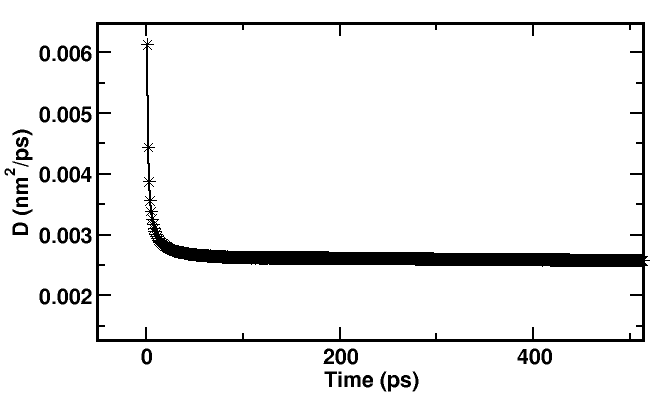
\includegraphics[height =7cm, width =7.33cm]{Chapter4/Diffusion_303.png}}
\subfigure[]{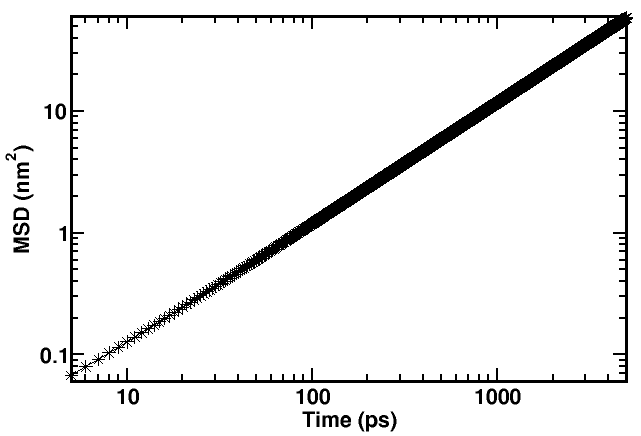
\includegraphics[height =7cm, width =7.32cm]{Chapter4/logorithm_msd.png}}
\caption[Plot of  MSD vs time  in logarithmic scale and the  diffusion coefficient nitric oxide.] {(a) Plot of Diffusion coefficient (D) = $\left\langle r^2(t)\right\rangle / 6\;t$ vs time of NO at 303 K. (b) Plot of MSD vs time in logarithmic scale for NO at 303 K. }
\label{diffusionno}
\end{center}
\end{figure}
%%%%%%%%%%%%%%%%%%

  The figure (\ref{diffusionno}) represents  (a) the  variation of diffusion coefficient (D) = $\left\langle r^2(t)\right\rangle / 6*t$  with  time and (b) the log-log plot of mean square displacement with time  for NO at temperature T = 303 K. From figure (\ref{diffusionno} a), we can say that at first the diffusion coefficient is high due to ballistic motion and later as time passes it remains constant. This constant portion of the graph gives the diffusion coefficient. The ballistic region is also  seen in figure (\ref{diffusionno} b) and is represented by the parabolic region of
 the graph very close to origin. In this case, the molecules at the beginning move swiftly in the holes present in the system thereby  showing higher value of diffusion coefficient. After certain time the molecules show uniform motion as a result of which we see the linear portion of the plot.
 
%%%%%%%%%%%%%%%%%%
\begin{figure}[h!]
 \centering
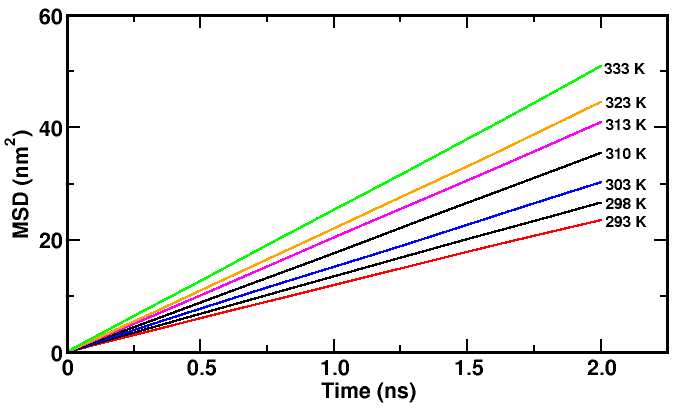
\includegraphics[scale=0.48]{Chapter4/msd_no_all.png}
\caption[Plot of MSD vs time of NO at different temperatures. ]{Plot of MSD vs time of NO at different temperatures, from 293 K to 333 K.}
\label{msdno}
\end{figure}
%%%%%%%%%%%%%%%%%%

 To obtain diffusion coefficient via MSD we plot the graph between mean square displacement with time. Figure (\ref{msdno}) shows the MSD plot of NO in water at different temperatures. Since the statistics is better due to higher averaging at the starting than towards the ending region, we take the certain portion which has the best statistics. We  fit the data linearly using \emph{grace}, the slope divided by 6 (equation \ref{Einstein}) gives the value of diffusion coefficient of the desired species under study. In our case, we have a simulation time of 200 ns and the best statistics for NO molecule is found within 2 ns which can also be justifiable from figure (\ref{diffusionno}) and is very small in comparison to simulation time this is due to lesser number of NO molecules. For water molecules best statistics is found within 5 ns due to larger number of water molecules as in figure (\ref{msdalkanewater}). The values of the self-diffusion coefficient of NO and water obtained from MSD plot are presented in table (\ref{diffusiontable}).

%%%%%%%%%%%%%%%%%%
 \begin{figure}[h!]
 \begin{center}
 \subfigure[]{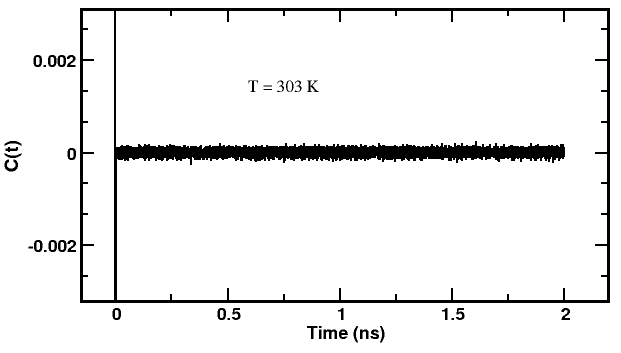
\includegraphics[height =7cm, width =7.32cm]{Chapter4/vac_303.png}} 
 \subfigure[]{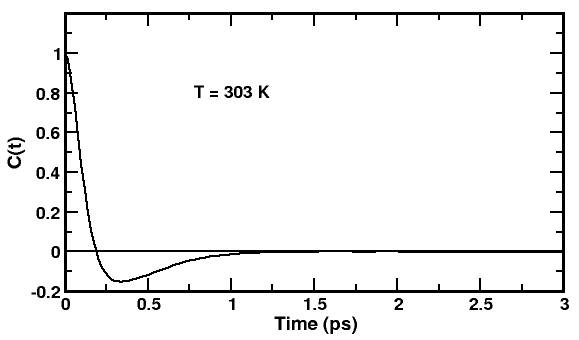
\includegraphics[height =7cm, width =7.32cm]{Chapter4/normalized_vac.png}}
 \caption[ Plot of velocity autocorrelation function with time for NO in water.] { Velocity autocorrelation function for NO (a) C(t) = $\left\langle v_i(t).v_i(0) \right\rangle_{i \in \alpha}$ vs time  (b)  Normalized C(t) = $\left\langle v_i(t).v_i(0) \right\rangle_{i \in \alpha}$  vs time at 303 K. }
 \label{velauto}
 \end{center}
 \end{figure}
 %%%%%%%%%%%%%%%%%%
 Figures (\ref{velauto} a) and  (\ref{velauto} b)   show the variation of velocity autocorrelation function with
time and the normalized velocity autocorrelation function  truncated graph to few ps time to see the variation of the velocity correlation function at small time interval for NO at temperature T=303 K. We here look at the product of the two velocities at two instance that are apart by time $t$. If $t$ is very small, the velocity doesn't change very much. So, in the limit of small time $t$, the velocity
at time $0$ and the velocity at  time $t$ are going to be very similar, we can say that there is a correlation. As we move away in time, there is going to be no correlation. The velocity at time $0$ and the velocity at an instant that is very far away in time is not going to be
correlated. To calculate the self-diffusion coefficient, we integrate the graph (\ref{velauto}) and divide the result by 3 (equation \ref{vacf1}). The comparison of the values obtained by using  VACF method, MSD method and the references is shown in
table (\ref{diffusiontable}).

The mutual diffusion coefficient is estimated using Darken's relation (equation \ref{darken}). Our system consists of
$5$ NO and $280$ water molecules so the mole fraction for water is 0.982 and that of NO is 0.018. The values of the mutual diffusion coefficient obtained using equation (\ref{darken}) is also presented in table (\ref{diffusiontable}).
\begin{table}[H]
  \centering
  \caption[The simulated value of Diffusion coefficient of NO and H$_\mathrm{2}$O, and  the references for them. ]{The simulated value of Diffusion coefficient of NO and H$_\mathrm{2}$O, and also the references for them  (a~ \citep{wise1968diffusion}, b~\citep{easteal1989diaphragm}, c~\citep{zacharia2005diffusivity}, d~ \citep{malinski1993diffusion}, and e~\citep{Thapa2013}) as a
  function of temperature are listed. The mutual diffusion coefficients between the solute and solvent molecules are also mentioned.}
 \label{diffusiontable}
\resizebox {0.55 \textwidth }{!}{%
\begin{tabular}{|c| c| c| l| c| c| c|}
\hline 
\multicolumn{7}{|c|}{Diffusion Coefficient  (1 $\times$10$^{-\mathrm{9}}$ m$^\mathrm{2}$s$^{-\mathrm{1}}$)} \\ 
\hline 
Temperature (K) & \multicolumn{3}{c}{For NO} &\multicolumn{2}{|c|}{For H$_\mathrm{2}$O} &
Mutual-diffusion \\ \cline{2-6} & MSD & VACF  & Ref. & MSD &  Ref & \\ \hline 
293 & 2.28 & 2.31 & 2.07(a) & 1.98 & 2.02(b)  & 2.27  \\ \hline 
298 & 2.54 & 2.58 & 2.21(c) &   2.21 &   2.24(e) & 2.53  \\ \hline
303 & 2.73 & 2.73 & 3.96(a) & 2.42 & 2.59(b)  & 2.72 \\  \hline
310 & 3.05 & 3.06 & 3.00(c) &  2.80 &  & 3.04 \\ 
 &  &  & 3.30(d) &   &  &  \\ \hline
313 & 3.31 & 3.46 & 5.16(a) & 3.01 & 3.24(b) & 3.30 \\  \hline
323 & 3.87  & 4.06  & 9.34(a) & 3.60 & 3.96(b)  & 3.86  \\   \hline
333 & 4.66 &  4.60 & 13.6(a)& 4.33 & 4.77(b) & 4.65 \\ 
\hline 
\end{tabular}}
\end{table} 

Table (\ref{diffusiontable}) shows the self-diffusion coefficients of NO and H$_\mathrm{2}$O molecules from the present work along with the references and also reveals the mutual diffusion coefficients between them, at different temperatures. The comparison of the values from the table and also from other references explores that self-diffusion coefficients of water from the present work, in general,
come in very good agreement with the previous studies~ \citep{easteal1989diaphragm, Thapa2013, Poudyal2014, zacharia2005diffusivity}. The experimental and simulated values of self-diffusion coefficients are in good agreement with maximum  deviation of $9.22\%$  at 
333 K~ \citep{easteal1989diaphragm}. The simulated values of NO, on the other hands, show different attitude towards the references. They agree very well with the experiment performed by Zacharia et al.~\citep{zacharia2005diffusivity} at 298 K and 310 K, which represent the environmental temperature
and temperature of physiological importance, respectively. The diffusion coefficient of NO at 310 K also falls within 2$\%$ of the experimental work reported by Malinski et al.~\citep{malinski1993diffusion}. This trend of agreement is also true with the pioneer work performed by Wise and Houghton (cited in the table \ref{diffusiontable}, Ref.~ \citep{wise1968diffusion}) at low temperature (within 9.21 $\%$ at 293 K). However, the agreement with the Ref.~ \citep{wise1968diffusion} remain no  longer true as we move towards higher temperatures. The values presented by the authors at higher temperatures are abnormally high with reference to the present work and also with other similar molecules (by size and weight, diffusivity is sensitive to these parameters) like carbon monoxide (CO) and molecular 
oxygen (O$_\mathrm{2}$) mentioned by the same author/s~ \citep{wise1968diffusion, wise1966diffusion}. The authors on the paper claim that the higher diffusivity of NO can be described on the basis of their paramagnetic behavior, which, so far in our knowledge, has not been mentioned
by the following research works and also has not been incorporated in the present work which demands further work. Moreover, we have taken the Lennard-Jones optimized parameter at low temperatures~ \citep{zacharia2005diffusivity}.

 The diffusion coefficients of NO are obtained by two different methods; VACF and MSD. Table \ref{diffusiontable} shows that both the methods produce similar values, within maximum deviation of 5.0$\%$. The diffusion coefficient for both the solute and solvent
molecules increases with the enhanced temperature, which is due to the increase in the velocity of the molecules, as per relation of the thermal energy with temperature. Furthermore, as the density of the system decreases with increasing temperature, the space available for the nitric
oxide molecules to execute random-walk motion increases~\citep{Thapa2013}. Finally, based on these facts, the mean squared displacement increases and this change is incorporated by Einstein's relation to yield an increased self-diffusion coefficient. The RDF of  oxygen atoms of nitric oxide themselves $g_{ON-ON}(r)$  (figure \ref{rdfonon}) shows finite density of the particles in the region between the first and second peaks, which also hints the diffusion process of the molecules in the whole system.

 The mutual diffusion coefficient is calculated using Darken's relation (equation (\ref{darken})) and is  very close to that of self-diffusion coefficient of solute in the mixture due to low solute concentrations studied in this work.

Similarly, for the studied system CO in water,  the comparison of the value obtained by using velocity autocorrelation method (VACF), MSD method and experimental value is shown in table (\ref{diffusiontableco}). Figure \ref{msdco} represents the MSD plot of CO at different temperatures and the values of diffusivity obtained is  presented in table (\ref{diffusiontableco}).

%%%%%%%%%%%%%%%%%%
\begin{figure}[h!]
 \centering
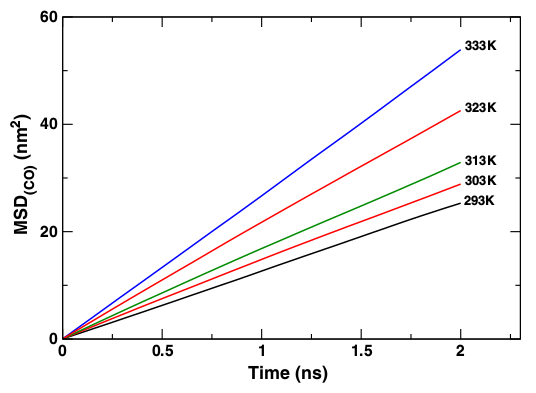
\includegraphics[scale=0.55]{Chapter4/msd_co_all.png}
\caption[Plot of MSD vs time of CO at different temperatures. ]{Plot of MSD vs time of CO at different temperatures, from 293 K to 333 K.}
\label{msdco}
\end{figure}
%%%%%%%%%%%%%%%%%%

 
 \begin{table}[H]
   \centering
   \caption[The simulated value and the experimental value of Self-Diffusion coefficient of CO
   molecule. ]{The simulated value and the experimental value of Self-Diffusion coefficient of CO  molecule as a  function of temperature are listed.}
  \label{diffusiontableco}
 \resizebox {0.65 \textwidth }{!}{%
 \begin{tabular}{|c| c| c| c|}
 \hline 
 \multicolumn{4}{|c|}{Diffusion Coefficient  (1 $\times$10$^{-\mathrm{9}}$ m$^\mathrm{2}$s$^{-\mathrm{1}}$)} \\ 
 \hline 
 Temperature (K) & \multicolumn{2}{|c|}{Simulated value} & Experimental Value~ \citep{wise1968diffusion} \\ \cline{2-3} 
 & MSD & VACF  &  \\ \hline 
 293 & 2.109 $\pm$ 0.018 & 2.053 & 2.03   \\ \hline 
 303 & 2.396$\pm$  0.135& 2.347 & 2.43   \\ \hline
 313 & 2.772$\pm$  0.062& 2.823 & 3.62 \\  \hline
 323 & 3.535$\pm$  0.162& 3.477 & 4.11  \\  \hline
 333 & 4.483$\pm$ 0.089& 4.587 & 5.68 \\  \hline 
 \end{tabular}}
 \end{table} 
 
 Table (\ref{diffusiontableco}) shows the simulated and experimental values of the self-diffusion coefficient of CO molecule at different temperatures. The simulated values of the  self-diffusion coefficient of CO using MSD method varies within 2$\%$ maximum
 in comparison to VACF method. From this we can infer that the simulated values estimated using two methods (i.e. MSD and VACF) are in good agreement. The self-diffusion coefficient estimated using both the methods varies within  15$\%$ to that of experimental value ~\citep{wise1968diffusion} except at temperatures T=313 K and T=323 K, which are more than 15$\%$. 
 
 The diffusion coefficient increases with the increase in temperature as expected.
 This is due to the increase in the velocity of the molecules because of the energy imparted to the molecules in accordance with the increase in temperature.  Also, the density of the system decreases with increasing temperature and hence increasing the space available for the carbon monoxide molecules to execute random-walk motion~\citep{Thapa2013}. Because of these, the mean squared displacement increases which by Einsteins relation yields an increased self-diffusion coefficient.
 
 For our system CO in water, the system consists of only 5 CO molecules  and 280 water molecules. Since the system  consists of 5 CO and 280 H2O molecules, the mole fraction of H2O is 0.982 and the mole fraction of CO  is 0.018.  The mutual diffusion coefficicnts of CO in water at different temperatures is presented in table (\ref{mutualdiffusionco}).
 
 \begin{table}[H]
 \centering
 \caption[The calculated value of mutual diffusion coefficient of Carbon monoxide in water.] {The calculated value of mutual diffusion coefficient of Carbon monoxide in water as a  function of temperature are listed.}
   \label{mutualdiffusionco}
 \resizebox {0.65 \textwidth}{!}{%
 \begin{tabular}{|c|c|c|c|}
 \hline 
 \multicolumn{4}{|c|}{Mutual Diffusion Coefficient of CO in H$_2O$  ($1 \times 10^{-9} \mathrm{m}^2 \mathrm{s}^{-1}$)} \\ 
 \hline 
 {Temperature (K)} &  \multicolumn{2}{|c|}{Self-Diffusion Coefficient} & {Mutual Diffusion Coefficient} \\ \cline{2-3}
  & For CO & For H$_2$O & \\ \hline
  293 & 2.130 & 1.980 & 2.127 \\ \hline
  303 & 2.400 & 2.420 & 2.400 \\ \hline
  313 & 2.770 & 2.932 & 2.773 \\ \hline
  323 & 3.530 & 3.520 & 3.530 \\ \hline
  333 & 4.480 & 4.145 & 4.474 \\ \hline
  \end{tabular}}
 \end{table}
 
From table (\ref{mutualdiffusionco}), we can infer that the mutual diffusion coefficient is nearer to  the diffusion coefficient of carbon monoxide. For the low solute concentrations
 studied in this work, the contribution to the mutual diffusion coefficient is nearly
 equal to the self-diffusion coefficient of the solute in the mixture. If the system
 is at infinite dilute condition then the mutual diffusion coefficient is equal to
 self-diffusion coefficient.
 
  %%%%%%%%%%%%%%%%%%
  \begin{figure}[h!]
  \begin{center}
  \subfigure[]{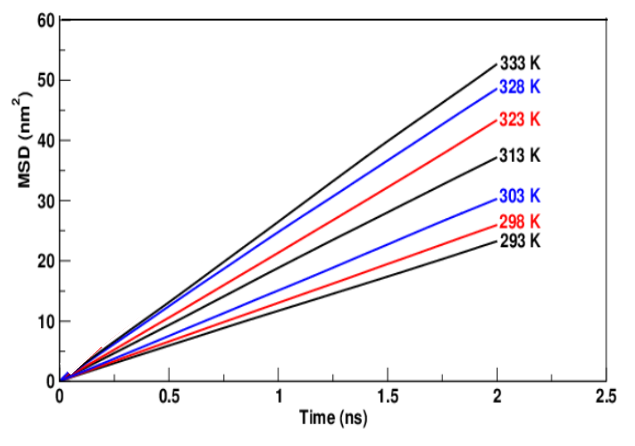
\includegraphics[height =7cm, width =7.32cm]{Chapter4/nitrogen_msd.png}} 
  \subfigure[]{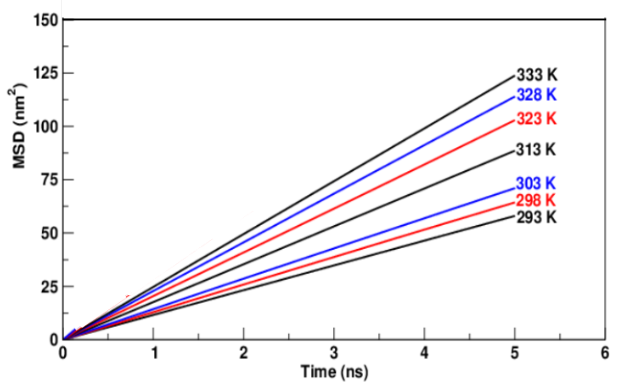
\includegraphics[height =7cm, width =7.32cm]{Chapter4/watern2_msd.png}}
  \caption[Plot of mean square displacement (MSD) vs time of nitrogen  and water.] {(a) Plot of mean square displacement (MSD) vs time of nitrogen molecules  in water at  different temperatures. (b) Plot of MSD vs time of water at different temperatures.}
  \label{msdnitrogenwater}
  \end{center}
  \end{figure}
  %%%%%%%%%%%%%%%%%%
 
 Figure (\ref{msdnitrogenwater}) shows the change in MSD of  the different species of the mixture (nitrogen and water)  at different temperatures. From the
 graph, we see that the MSD vary linearly with time as expected. Further with increase
 in temperature, the MSD also increases which is an indication that the diffusion coefficient must increase with increase in temperature. It is because, as temperature increases,
 the generated velocities of the water molecules also increases. Also since at higher 
 temperature, the density of the system decreases thereby increasing the space available for
 the molecules to execute random-walk. This cause MSD to increase and also diffusion
 coefficient increases.
  
 The values of diffusion coefficients of nitrogen in water at different temperatures as calculated
 by MSD and VACF methods  are tabulated in table (\ref{diffusiontablen2}).
 
 \begin{table}[H]
    \centering
    \caption[The simulated value and the experimental value of Self-Diffusion coefficient of N2
    molecule. ]{The simulated value and the experimental value of Self-Diffusion coefficient of N2  molecule as a  function of temperature are listed.}
   \label{diffusiontablen2}
  \resizebox {0.65 \textwidth }{!}{%
  \begin{tabular}{|c| c| c| c| c|}
  \hline 
  \multicolumn{5}{|c|}{Diffusion Coefficient  (1 $\times$10$^{-\mathrm{9}}$ m$^\mathrm{2}$s$^{-\mathrm{1}}$)} \\ 
  \hline 
  Temperature (K) & \multicolumn{2}{c|}{Simulated value} & \multicolumn{2}{c|}{Experimental Values} \\ \cline{2-5} 
  & MSD & VACF  &  \citep{ferrell1967diffusion}  & \citep{verhallen1984diffusion}  \\ \hline 
  293 & 1.922 $\pm$ 0.026 & 1.971 & -- & 2.00  \\ \hline 
  298 & 2.152$\pm$  0.004& 2.083 & 2.01 & -- \\ \hline
  303 & 2.530$\pm$  0.005& 2.380 & -- &  2.60 \\ \hline
  313 & 3.106$\pm$  0.082& 3.027 & 2.83 & 3.30 \\ \hline
  323 & 3.607$\pm$  0.103 & 3.763 & -- & 4.10\\  \hline
  328 & 4.044$\pm$  0.166 & 4.050 & 3.80 &-- \\  \hline
  333 & 4.411$\pm$ 0.063 & 4.240 & -- &  4.90\\  \hline 
  \end{tabular}}
  \end{table} 
  
 Table (\ref{diffusiontablen2}) presents the self diffusion coefficient of nitrogen obtained by Einstein’s relation (MSD method) and velocity auto-correlation function (VACF)  method in the present work  and that experimentally observed values in different works. The values of self-diffusion  coefficient of N2 is almost same with maximum deviation of about 3$\%$ at temperature 323 K when calculated using MSD method and VACF method. The values of diffusion coefficients found by Ferrel et al. ~\citep{ferrell1967diffusion} are in agreement with that found by current simulation method within 10$\%$ in MSD method and are within 7$\%$ in VACF method. Similarly the  diffusion coefficients found by Verhallen et al.~\citep{verhallen1984diffusion} are in agreement within 12$\%$ in MSD
 method and within 14$\%$ when calculated using VACF method. 
 
 From the table it is seen that the diffusion coefficient of nitrogen increases with in-
 crease in temperature. As temperature increases, the generated velocities increases due
 to the energy imparted to the molecules, which thereby increase the diffusion coefficient.
 Also, as the density increase with increase in temperature, so the space available for
 random-walk of nitrogen molecules increases and the molecules can diffuse readily.
 
 For the system N2 in water, the system consists of only 5  molecules of nitrogen  and 265 molecules of water. For this system,  the mole fraction
 of H2O is 0.9815 and the mole fraction of N2 is 0.0185. The mutual diffusion coefficients
 of N2 in water at different temperatures is presented in table (\ref{mutualdiffusionn2}). 
 
\begin{table}[H]
 \centering
 \caption[The calculated value of mutual diffusion coefficient of Carbon monoxide in water.] {The calculated value of mutual diffusion coefficient of Carbon monoxide in water as a  function of temperature are listed.}
   \label{mutualdiffusionn2}
 \resizebox {0.65 \textwidth}{!}{%
 \begin{tabular}{|c|c|c|c|}
 \hline 
 \multicolumn{4}{|c|}{Mutual Diffusion Coefficient of N2 in H$_2O$  ($1 \times 10^{-9} \mathrm{m}^2 \mathrm{s}^{-1}$)} \\ 
 \hline 
 {Temperature (K)} &  \multicolumn{2}{|c|}{Self-Diffusion Coefficient} & {Mutual Diffusion Coefficient} \\ \cline{2-3}
  & For N2 & For H$_2$O & \\ \hline
  293 & 1.922 & 1.934 & 1.922 \\ \hline
  298 & 2.152 & 2.146 & 2.152 \\ \hline
  303 & 2.530 & 2.365 & 2.526 \\ \hline
  313 & 3.106 & 2.955 & 3.102 \\ \hline
  323 & 3.607 & 3.426 & 3.604 \\ \hline
  328 & 4.044 & 3.799 & 4.039 \\ \hline
  333 & 4.411 & 4.127 & 4.406\\ \hline
  \end{tabular}}
 \end{table}
 
 From table (\ref{mutualdiffusionn2}), it is seen that the mutual diffusion coefficient of the system is almost equal to the self diffusion coefficient of nitrogen. It is because of the large number of solvent molecules (water)  in our system.
 
%%%%%%%%%%%%%%%%%%%%%%%%%%%%%%%%%%%
\subsection{Diffusion Coefficient as a function of temperature }
%%%%%%%%%%%%%%%%%%%%%%%%%%%%%%%%%%%
The diffusion do depends on temperature as seen in previous section. So, like chemical
reactions, diffusion is also a thermally activated process. Diffusion coefficients of a system generally depends strongly on temperature, being low at low temperatures and are found to be increased with increase in temperature. Temperature variations in diffusivity is explained by the  Arrhenius-type exponential relationship~ \citep{mehrer2007}.
\begin{equation} \label{Arrhenius_equation}
\mathrm{D}= \mathrm{D}_0~\mathrm{exp}\left(-E_a/R \; T\right)
\end{equation}
which can be expressed as 
\begin{equation}
ln D = ln D_0 - E_a/R\;T
\label{arrentype}
\end{equation}
where, D$_0$ denotes the pre-exponential factor, also called frequency factor, E$_a$ is the activation energy for diffusion, $T$ is the absolute temperature, R =N$_A$ k$_B$ is molar gas constant whose value is is $8.31~ \mathrm{J ~{mol}^{-1} K^{-1}}$, N$_A$ is Avogadro constant whose value is $6.023 \times 10^{23}$ and k$_B$ is the Boltzmann constant whose value
is $1.38 \times 10^{-23}\; J K^{-1}$. Both E$_a$ and D$_0$ are called the activation parameters of diffusion.

The activation energy of diffusion process ~\citep{mehrer2007}
\begin{equation}
E_a = -R \frac{\partial\mathrm {ln}D}{\partial (1/T)}
\end{equation}
corresponds to negative slope of the Arrhenius diagram. The intercept of the extrapolated Arrhenius line for T$^{\mathrm{-1}} \Longrightarrow 0 $ yields the pre-exponential factor D$_\mathrm{0}$. In an Arrhenius diagram the logarithm of the diffusivity is plotted versus the reciprocal of absolute temperature. 

For the studied systems, the simulated and experimental diffusivity of constituents of the system  have been fitted to Arrhenius-type expression equation (\ref{arrentype}) by least
squares method, the pre-exponential constant $\mathrm{D_0}$ and the activation energy $\mathrm{E_a}$ are reported for the corresponding constituents of the studied systems.

\begin{table}[H]
\centering
 \caption[Activation energies and pre-exponential factors for diffusion of various studied alkane-water system.] {Activation energies and pre-exponential factors for diffusion of various studied alkane-water system.}
  \label{activation_energy}
\resizebox {0.65 \textwidth } {!}{%
\begin{tabular} {|c|  c| c| }  \hline
 system & $E_a$ (kJ $mol^{-1}$) & $D_0 \times 10^7 m^2/s $  \\ \hline
CH4-H2O & 15.13 &  7.00 \\ \hline 
C2H6-H2O & 16.18  & 11.86 \\ \hline  
C3H8-H2O & 17.81  & 18.67 \\  \hline
C4H10-H2O & 18.38  & 22.63 \\  \hline
H2O & 15.59  & 13.12 \\\hline
\end{tabular}} 
\end{table} 

 Figure(\ref{arrhenius_alkane})  shows the temperature dependence of diffusion coefficient of alkane in water. As the simulation  data fit to the equation (\ref{Arrhenius_equation}), the temperature dependence of diffusion coefficient follows Arrhenius  behavior. From figure (\ref{arrhenius_alkane}), it is seen that the diffusion coefficients increase with increase in temperatures. This could be due to the fact that at higher temperature the difference in the density of the system (i.e. alkane and water) increases with  increase in temperature (see table (\ref{density_box})).
\noindent Figure (\ref{arrhenius_water}) shows the temperature dependence of diffusion coefficient of water in the system containing water and alkane. Figure (\ref{arrhenius_water}) explicitly shows the temperature dependence of diffusion coefficient of water also follows Arrhenius behavior.

%%%%%%%%%%%%%%%%%%
\begin{figure}[h!]
 \centering
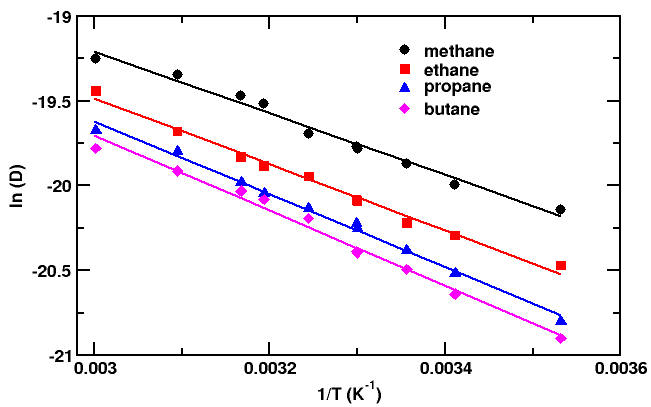
\includegraphics[scale=0.55]{Chapter4/arre_alkane.png}
\caption[Arrhenius plot of the simulated values of binary diffusion coefficients of alkane in water.] {Arrhenius plot of the simulated values of binary diffusion coefficients of alkane.}
\label{arrhenius_alkane}
\end{figure}
%%%%%%%%%%%%%%%%%%

%%%%%%%%%%%%%%%%%%
\begin{figure}[h!]
\centering
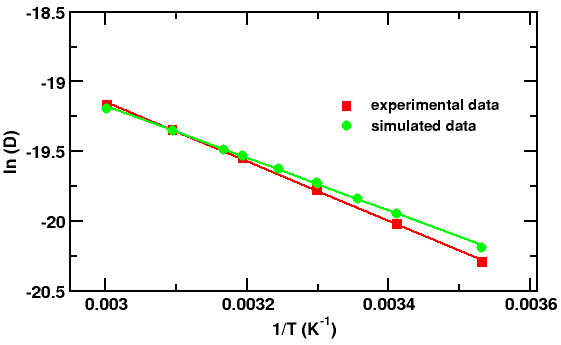
\includegraphics[scale=0.65]{Chapter4/arrwat.png}
\caption[Arrhenius plot of the simulated and experimental values of self diffusion coefficients of  water.] {Arrhenius plot of the simulated and experimental values of self diffusion coefficients of water.}
\label{arrhenius_water}
\end{figure}


\begin{table}[H]
 \centering
 \caption[ Activation Energy for diffusion of the studied systems.] { Activation Energy for diffusion  of the studied systems ( NO, CO, N2 in water)  and the corresponding experimental values.}
   \label{Activation_energy}
 \resizebox {0.65 \textwidth}{!}{%
 \begin{tabular}{|c|c|c|c|}
 \hline 
 \multicolumn{4}{|c|}{ Activation Energy $E_a$ (kJ $mol^{-1}$) } \\ 
 \hline 
 System & \multicolumn{2}{|c|}{Simulated Values From } & Experimental Values \\ \cline{2-3}
  & MSD & VACF &  \\ \hline
  NO-H2O & 14.28 & 14.32 & 19.50 \\ \hline
  CO-H2O & 15.43 & 16.02 & 20.93 \\ \hline
  N2-H2O & 15.26 & 15.32 & 17.25, 18.26\\ \hline
  H2O    &  15.87 & -- & 17.41 \\ \hline
  \end{tabular}}
 \end{table}
 
 %%%%%%%%%%%%%%%%%%
 \begin{figure}[h!]
 \centering
   \subfigure[]{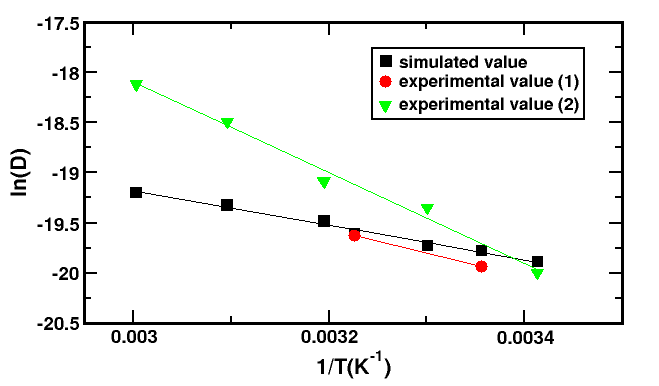
\includegraphics[width=13 cm,height= 9 cm]{Chapter4/arren_no.png}}
 \subfigure[]{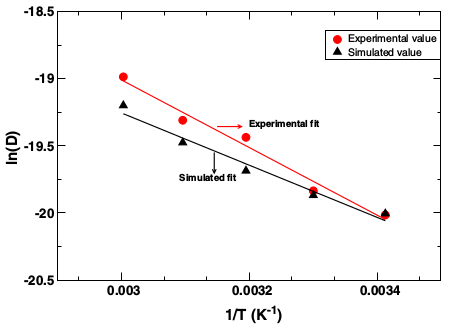
\includegraphics[width=13 cm,height= 9 cm]{Chapter4/arrene_co.png}}
   \caption[Arrhenius plot of the simulated  and experimental value of diffusion coefficients of    nitric oxide and carbonmonoxide in water.]{Arrhenius plot of the simulated  and experimental value of diffusion coefficients of  (a) nitric oxide in water and (b) carbonmonoxide in water.}
 \label{arrenewsplotall}
 \end{figure}
 %%%%%%%%%%%%%%%%%%
 


%%%%%%%%%%%%%%%%%%%%%%%%%%%%%%%%%%%
\section{Diffusivity and mobility of alkali and halide ion in water}
\label{ions}
%%%%%%%%%%%%%%%%%%%%%%%%%%%%%%%%%%%
In this section, we present and discuss the structural and dynamical properties of the studied system. The structural properties is studied with the help of  the radial distribution function(RDF) and ion-hydration number $N_H$, and the dynamic propeties is studied with the help of   diffusivity and mobility  of solute (ions) in   solvent TIP3P water (Section \ref{halide_diffusion}). 


%%%%%%%%%%%%%%%%%%%%%%%%%%%%%%%%%%%
\subsection {Structure of the Ion-water System}
%%%%%%%%%%%%%%%%%%%%%%%%%%%%%%%%%%%

Radial distribution function (RDF)  gives the information on the structure of the system. The  radial distribution function $g(r)$, defines the probability of finding a particle at a distance $r$ from a reference  particle of the system.  For a crystal, it exhibits a sequence of peaks at positions corresponding to shells around a given atom. For a  liquid, RDF exhibits its major peak close to the average atomic separations of neighbouring atoms and oscillates with less pronounced peaks at larger distances. The magnitude of the peaks decays exponentially with distances as $g(r)$ approaches 1 ~\citep{mcquarrie2000, Ercolessi1997}.

We have used radial distribution function and ion-hydration number to characterize the structure of the system. We have evaluated  RDF $g(r)$ of the ion-oxygen and oxygen-oxygen atoms of the water molecules in the studied system.

%%%%%%%%%%%%%%%%%%
 \begin{figure}[h!]
 \centering
   \subfigure[]{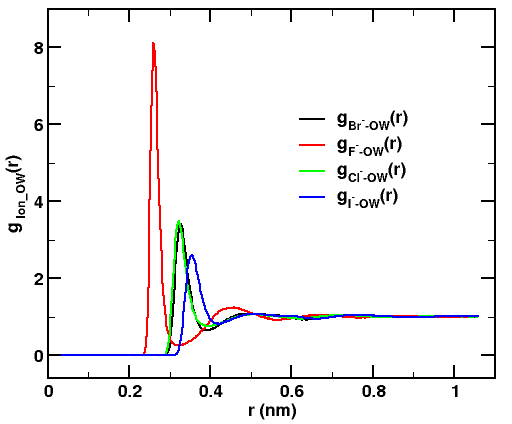
\includegraphics[width=12 cm,height= 8 cm]{Chapter4/rdf_all_anion.png}}
 \subfigure[]{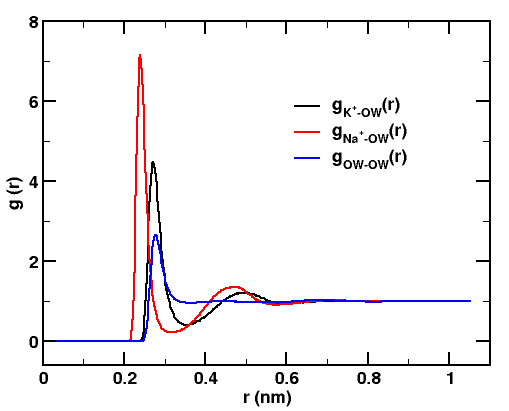
\includegraphics[width=12 cm,height= 8 cm]{Chapter4/rdf_all_cations.png}}
   \caption[Ion-Oxygen and Oxygen-Oxygen radial distribution function $\mathrm{g_{Ion-OW}}(r)$ of the alkali and halide ions in water.] {Radial Distribution functions of ions-oxygen  (a)  Anion (halide ion)-Oxygen  (b)  Cation (alkali ion)-Oxygen and Oxygen-Oxygen of alkali and halide ions in water at 298.15 K.}
 \label{rdfanion}
 \end{figure}
 %%%%%%%%%%%%%%%%%%

 Figure (\ref{rdfanion}) represents the RDF of oxygen atoms of water molecules and halide anions  and alkali cations of the studied system at 298.15 K. The ion-hydration number $N_H$ in the primary shell was calculated from the ion-oxygen distribution functions $g_{io}(r)$ as ~ \citep{mcquarrie2000}:
\begin{equation}
N_H = \int_0^{r_{min}} 4~ \pi ~\rho~ g_{io}(r)~r^2 dr
\end{equation}
Where $r_{min}$ is the radius of the coordination shell (location of the RDF minima) and $\rho$ is the number density. The detail of the structural properties along with the ion-hydration number  is provided in table(\ref{rdfowowtable}).

In table (\ref{rdfowowtable}) the 
ER stands for Excluded Region. The values of excluded region increases with the increase in mass of the anions and also for cations.  The value of $\sigma$ for OW-OW is  0.315061 nm, and the van der Waals radius (2$^{\mathrm{1/6}}\sigma$) is 0.35364 nm~ \citep{jorgensen1983comparison}. The table (\ref{rdfowowtable}) shows that excluded region is (0.244 $\pm$ 0.002 nm). It also shows that the excluded region is smaller than the van der Waals radius which indicates the contribution from other potentials in addition to the van der Waals potential~\citep{Pokhrel2016}.

\begin{table}[H]
 \centering
 \caption[The detail of the  structural properties along with the ion-hydration number for alkali-halide ions in water.] {Positions and Magnitudes at Maxima and
Minima of Solute-Oxygen $g_{io}$ and Oxygen-Oxygen Radial
Distribution Functions $g_{oo}$ at 25$^{\circ}$C and the ion-hydration number and co-ordination  of oxygen atoms of the water. }
\label{rdfowowtable}
\resizebox {0.95 \textwidth }{!}{%
\begin{tabular}{ |c |c| c |c |c |l |c |c| c| c |c|}
\hline 
  &  & \multicolumn{2}{|c|}{first max} & \multicolumn{3}{c|}{first min }  &\multicolumn{2}{c|}{second max } & 
\multicolumn{2}{c|}{second min } \\ \cline{3-4} \cline{5-6} \cline{7-11}
 {Ion} & ER  & $r_{max}$  & $g_{io}(r)$ & $r_{min}$  & $g_{io}(r)$ & $N_H$  & $r_{max}$  & $g_{io}(r)$ & $r_{min}$  & $g_{io}(r)$   \\ \hline  
$F^-$ & 0.238 & 0.262 & 8.056 & 0.322 & 0.248 & 6.8  & 0.458 & 1.234 & 0.562 & 0.909 \\ \hline
$Cl^-$ & 0.286 & 0.322 & 3.470 & 0.394 & 0.7611 & 7.8 & 0.5072  &   1.0646 & 0.6167 & 0.948  \\ \hline
$Br^-$ & 0.293 & 0.326 & 3.4185 & 0.390 & 0.6416 & 8.2 &  0.496  &1.077 & 0.6261 & 0.924 \\ \hline
$I^-$ & 0.312 & 0.356 & 2.599 & 0.420 & 0.8124 & 9.1 &0.5121 & 1.07 & 0.658 & 0.9439 \\ \hline
$Na^+$ & 0.212 & 0.240 & 7.126 & 0.314 & 0.2148 & 5.6 & 0.474 & 1.324 & 0.579 & 0.9074 \\ \hline
$K^+$ & 0.239  & 0.272  & 4.264 & 0.358 & 0.4069  & 6.8 & 0.490 & 1.204 & 0.596 & 0.92517  \\ 
\hline 
{Water} & ER  & $r_{max}$  & $g_{oo}(r)$ & $r_{min}$  & $g_{oo}(r)$ & $N_C$  & $r_{max}$  & $g_{oo}(r)$ & $r_{min}$  & $g_{oo}(r)$   \\ \hline
$H_2O$ & 0.244  & 0.278  & 2.690 & 0.361   & 0.938 & 5.4  & 0.450  & 0.990546 & 0.5848  & 0.948   \\ \hline 
\end{tabular}}
\end{table} 

%%%%%%%%%%%%%%%%%%%%%%%%%%%%%%%%%%%
\subsection {Diffusivity, Mobility and Friction Coefficients}
%%%%%%%%%%%%%%%%%%%%%%%%%%%%%%%%%%%
The diffusivity of the solvated ion  is determined by   using Einstein's relation (MSD method) [Eq. (\ref{Einstein})] and Green-Kubo formula (VACF method) [Eq.(\ref{vacf1})]  and that of water is determined by using Einstein's relation (MSD method) [Eq. (\ref{Einstein})] only.

%%%%%%%%%%%%%%%%%%
\begin{figure}[h!]
 \centering
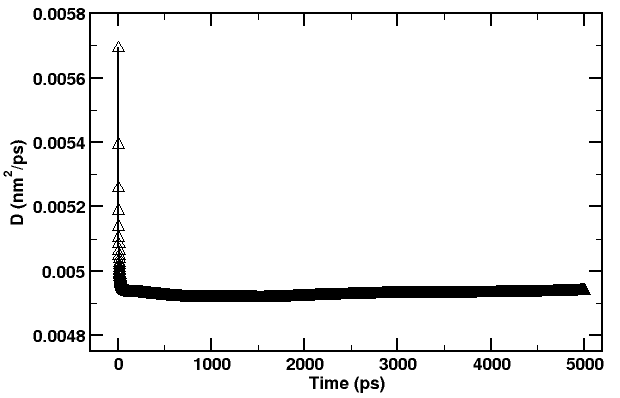
\includegraphics[scale=0.35]{Chapter4/Diffusion.png}
\caption[Diffusion coefficient  vs time of TIP3P water from MSD. ]{ Diffusion coefficient (D) = $\left\langle r^2(t)\right\rangle / 6\;t$ vs time of TIP3P water from MSD  at 298.15 K. }
\label{diffusionvstime1}
\end{figure}
%%%%%%%%%%%%%%%%%%

 The figure (\ref{diffusionvstime1}) shows the variation of diffusion coefficient (D) = $\left\langle r^2(t)\right\rangle / 6*t$  with
time for TIP3P water at temperature T = 298.15 K. In  figure (\ref{diffusionvstime1}) we  have taken the time up to 5 ns while calculating diffusion coefficient. At first the diffusion coefficient is high due to ballistic motion and later as time passes it remains constant.  At the beginning, the molecules  move swiftly in the holes present in the system thereby showing higher value of diffusion coefficient. After certain time the molecules show uniform motion and attain steady state  as a result of which we see the linear portion of the plot. The value of diffusion coefficient of TIP3P water at 298.15 K is found to be  $(4.98 \pm 0.17) \times 10^{-9} m^2s^{-1}$ which is in close agreement with  the previously reported value  $(5.06 \pm 0.09) \times 10^{-9} m^2s^{-1}$~ \citep{mahoney2001diffusion}. This value is greater than the experimental value of the diffusion coefficient of water $2.30 \times 10^{-9} m^2s^{-1}$~ \citep{mills1973self}. This shows that TIP3P model of water overestimate the diffusion coefficient of water. 

%%%%%%%%%%%%%%%%%%
\begin{figure}[h!]
 \centering
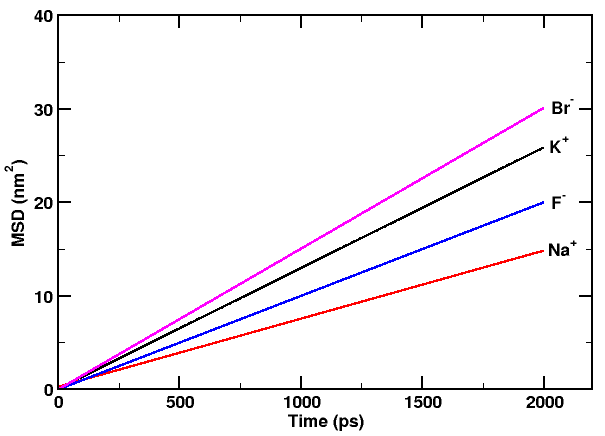
\includegraphics[scale=0.38]{Chapter4/msd_4.png}
\caption[Mean square displacement  of the cations   and anions in water. ]{ Mean square displacement  of the cations $Na^+$, $K^+$  and anions $F^-$ $Br^-$ in water  at 298.15 K. }
\label{msd-4}
\end{figure}
%%%%%%%%%%%%%%%%%%

 To obtain diffusion coefficient via MSD we plot the graph between mean square displacement with time. Figures (\ref{msd-4}) show the MSD plot of the cations $Na^+$, $K^+$  and anions $F^-$ $Br^-$ in water  at 298.15 K. We  fit the data linearly with method of least squares  using \emph{grace}, the slope divided by 6 (equation \ref{Einstein}) gives the value of diffusion coefficient of the desired species under study. Though the time of simulation of the system is 100 ns, the best statistics for the ions  is found within 2 ns. For water molecules best statistics is found within 5 ns due to larger number of water molecules.

%%%%%%%%%%%%%%%%%%
\begin{figure}[h!]
 \centering
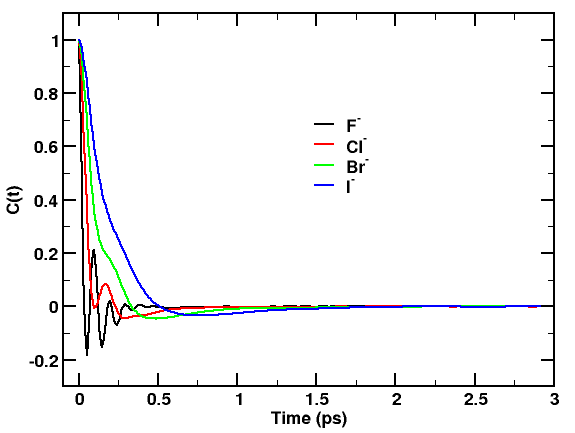
\includegraphics[scale=0.38]{Chapter4/vacf_halide.png}
\caption[Normalized velocity auto-correlation function   vs  time of halide ions.] { Normalized velocity auto-correlation function  $ c (t) = \left\langle  \textbf{v}_i(t).\textbf{v}_i(0) \right\rangle $ vs   time of halide ions at 298.15 K. }
\label{normalize_velacc}
\end{figure}
%%%%%%%%%%%%%%%%%%

 Figure (\ref{normalize_velacc}) shows the variation of  normalized velocity autocorrelation function with time  truncated graph to few ps time to see the variation of the velocity correlation function at small time interval for halide ions $F^-$ $Cl^-$ $Br^-$ $I^-$ in water at 298.15 K.  We Here  we see  the product of the two velocities at two instance
that are apart by time $t$. The result in \ref{normalize_velacc} 
shows a gradual change from oscillatory to monotonic decay as the ion size of the halide increases. An oscillatory behavior of the velocity autocorrelation function for the small ion can be understood as a result of the oscillatory motion of the ion within the molecular complex. A small ion is firmly solvated by the surrounding solvent molecules, and makes a kind of molecular complex with those solvent molecules~\citep{tobias2001surface}. Since the lifetime of such a complex is expected to be substantial for a sufficiently small ion, the small ion will continue to oscillate within that complex for some time. The relaxation time of the oscillatory feature in the velocity autocorrelation function may reflect the lifetime of that complex there is going to be no correlation~ \citep{chong1999dynamics, koneshan1998solvent}.  

 The diffusion coefficients of ions  are calculated independently from MSD and VACF using  equations (Eq.\ref{Einstein} and Eq. \ref{vacf1}). The diffusion coefficient of water is calculated from MSD using Eq. \ref{Einstein}. The  mobility is evaluated by equation (\ref{mobility}) and friction coefficient is calculated by equation (\ref{friction}). The calculated values of  ion diffusion coefficients , ion mobilities and friction coefficients of the ions are collected in table (\ref{diffusion_table1}). 
 
\begin{table}[H]
 \centering
 \caption[Diffusion Coefficients, Mobilities, and Friction Coefficients  of
 Solutes (alkali-halide ions) in water.] {Diffusion Coefficient $D$, Mobilities $\mu$, and Friction Coefficients $\xi$ of alkali-halide ions in water at 298.15 K Calculated from the Mean Square Displacements, Velocity Autocorrelation Functions and the reference (Ref.~ \citep{lide2009crc})}
\label{diffusion_table1}
\resizebox {0.65 \textwidth }{!}{%
\begin{tabular}{ |c| c| c| c| c| c| c| c | }
\hline 
  &  \multicolumn{3}{c|}{$D (\times 10^{-9} ~ m^2s^{-1}$) } &  \multicolumn{2}{c|}{$\mu (\times 10^{-8} m^2V^{-1}s^{-1}$)  } &  \multicolumn{2}{c|} {$\xi (\times 10^{-12} kgs^{-1}$ }  
 \\ \cline{2-4} \cline{5-6} \cline{7-8}
 {Ion}   & MSD  & VACF & Ref.  &   MSD  & VACF  &  MSD & VACF   \\ \hline  
$F^-$  & 1.42 &	 1.42 & 1.475 &  5.52 & 5.52  &  2.90 & 2.90  \\ \hline 
$Cl^-$ & 2.13 &    1.99 & 2.032 &  8.28 & 7.74 &  1.93 & 2.07  \\ \hline 
$Br^-$  & 2.32  &   2.08 & 2.080 & 9.02 & 8.08 &  1.77 & 1.98   \\ \hline 
$I^-$  & 2.24	& 2.06 & 2.045 &  8.71 & 8.01 &  1.84& 2.00 \\ \hline 
$Na^+$  & 1.36	& 1.36 & 1.334 &  5.29  &5.29  &  3.06 & 3.06   \\  \hline 
$K^+$   & 1.98  &   2.10 & 1.957 &  7.70 & 8.16 &  2.08 & 1.96  \\ 
 \hline 
\end{tabular}}
\end{table}

 Table (\ref{diffusion_table1}) shows the estimated values of diffusion coefficients of ions ($F^-$, $Cl,^-$, $Br^-$, $I^-$,$na^+$, $K^+$)  in water  at 298.15 K along with the references. The comparison of the values from the table with the  reference shows  that diffusion coefficients of ions  from the present work, in general, come in very good agreement with the experimental values~ \citep{lide2009crc}. The experimental and simulated values of diffusion coefficients are in good agreement with maximum  deviation of $11.53\%$  for $Br^-$ ion. The diffusion coefficients of ions  are obtained by two different methods; VACF and MSD. Table \ref{diffusion_table1} shows that both the methods produce similar values, within maximum deviation of 8.0$\%$. 


%%%%%%%%%%%%%%%%%%%%%%%%%%%%%%%%%%%
\section{Lighter alkanes in polar and amphiphilic environment} \label{solvation}
%%%%%%%%%%%%%%%%%%%%%%%%%%%%%%%%%%%

Hydrophobic interactions in between non-polar solutes on liquid media represents the model system for protein folding and its denaturation in living creatures. Different solutes and solvents have differences in their molecular size and structural arrangement which affect the nature of interactions in between solute particles~\citep{Sobolewski2007}. Using the computational  details described in the section \ref{alkane_solvation}, free energy of solvation calculations  were carried out in a  cubic box in infinite dilution for two separate systems: (i) 596 TIP3P water molecules and 1 OPLS-AA alkane (methane, ethane, propane and n-butane) molecule (ii) 354 OPLS-AA methanol  and 1 OPLS-AA alkane (methane, ethane, propane and n-butane) molecule. The free energy of solvation of alkanes in different solvent environments, water and methanol have been  estimated by Eq.\label{helmoltzfeee}. The extent to which Hamiltonian of the system has been perturbed is measured by the free energy change of transforming a system from state A ($\lambda=0$) to state B ($\lambda= 1$), $\Delta A$, as a function of a coupling parameter, $\lambda$. For decoupling van der Waals  interactions,  we used  an equidistant $\lambda$ spacing of 21 different $\lambda$'s from 0 to 1.  Thus, the free energy change from $\lambda = 0$ to $\lambda = 1$ is simply the sum of the free energy changes of each pair of neighboring $\lambda$ simulations. The free energy changes of each pair of neighboring $\lambda$ and the cumulative free energy change which is negative of free energy of solvation of butane in water is shown in figure (\ref{freeintegral}).


%%%%%%%%%%%%%%%%%%
\begin{figure}[h!]
 \centering
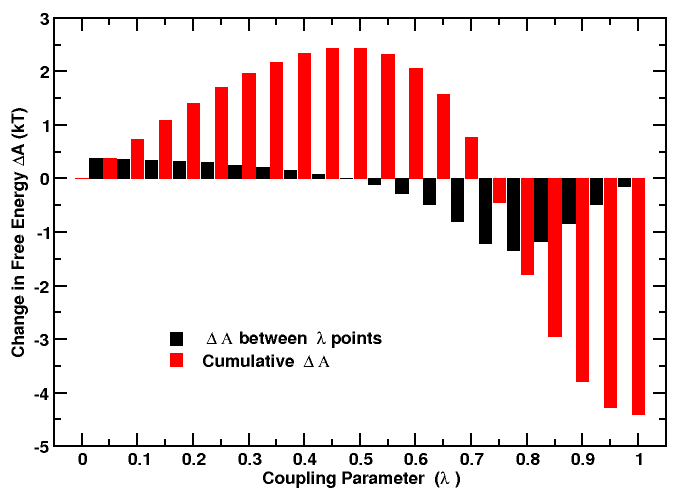
\includegraphics[scale=0.38]{Chapter4/free_energy_butane.png}
\caption[Difference in free energy  and cumulative free energy difference  for different lambda points for simulation of butane in water.] { Difference in free energy ($\Delta A$) and cumulative free energy difference ($\Delta A$) for different $\lambda$ points for simulation of butane in water at T = 300 K}
\label{freeintegral}
\end{figure}
%%%%%%%%%%%%%%%%%%
 
 
The calculated  values of solvation free energy of alkane (methane, ethane, propane, n-butane) in water  and  methanol along with the references (if available) at different temperatures are presented in table (\ref{freeenergy_table}). There is good agreement between experimental values at 298 K  and calculated values at 300 K of the solvation free energy of alkanes in water within 15 \%  error, but at higher temperatures there is no available experimental results. And there is no experimental available result for solvation free energy of alkanes in methanol.

\begin{table}[H]
 \centering
 \caption[Free Energy of solvation of light alkanes in water at different temperatures.] {Calculated and available experimental valus of   solvation free energies ($\mathrm{kJ mol^{-1}}$ ) of light alkanes (methane, ethane, propane, n-butane) in water and methanol at different temperatures.}
\label{freeenergy_table}
\resizebox {0.62\textwidth }{!}{%
\begin{tabular}{ |c| c| c | c | c  | c |  }
\hline 
    &  &    \multicolumn{2}{c|}{Water }   & \multicolumn{2}{c|} {Methanol } 
 \\ \cline{3-4} \cline{5-6} 
 {Molecule} & T (K)   & Calculated &   Expt.(298.15K)~\citep{ben1984solvation} &  Calculated &   Ref. \\ \hline  
 & 275 	 & 8.33 $\pm$ 0.05 & ---   & 2.94 $\pm$ 0.02 & ---  \\ 
  & 300 &	 9.08 $\pm$ 0.12 & 8.08   &  3.05 $\pm$ 0.10 & ---  \\
 Methane  &  325 &  10.01 $\pm$ 0.14  & ---  &  3.36 $\pm$ 0.01 & ---\\  
  & 350 &	 10.32 $\pm$ 0.09 & ---  &   3.58 $\pm$ 0.03 & --- \\ 
  & 375 &	  10.63 $\pm$ 0.07 & --- &   3.79 $\pm$ 0.05 & --- \\ \hline  
  & 275 &	  8.22 $\pm$ 0.14 & ---  & 0.20 $\pm$ 0.15 & ---  \\ 
  & 300 &	  9.02 $\pm$ 0.19 & 7.41  &  0.70 $\pm$ 0.12 & ---  \\
  Ethane   &  325 &  11.12 $\pm$ 0.07 & ---  &  0.90 $\pm$ 0.10 & ---\\  
  & 350 &	 11.20 $\pm$ 0.10 & ---  &   0.99 $\pm$ 0.10 & --- \\ 
  & 375 &	 11.52 $\pm$ 0.10 & --- &   1.01 $\pm$ 0.07 & --- \\ \hline  
  & 275 &	 8.77 $\pm$ 0.14 & ---  &  -2.73 $\pm$ 0.21 & ---  \\ 
  & 300 &	  9.61 $\pm$ 0.21 & 8.28  &  -1.28 $\pm$ 0.30 & ---  \\
  Propane  &  325 &	 11.27 $\pm$ 0.08 & ---  & -0.93 $\pm$ 0.16 & ---\\  
  & 350 &	  11.80 $\pm$ 0.06 & ---  &   --- & --- \\ 
  & 375 &	   12.70  $\pm$ 0.02 & --- &   --- & --- \\ \hline  
  & 275 &	  9.10 $\pm$ 0.13 & ---  &  -4.92 $\pm$ 0.19 & ---  \\ 
  & 300 &	  10.99 $\pm$ 0.18 & 9.03  &  -3.77 $\pm$ 0.18 & ---  \\
 n-Butane  &  325 &  11.82 $\pm$ 0.11  &---  &  -3.60 $\pm$ 0.19 & ---\\  
  & 350 &	  12.95 $\pm$ 0.20 & ---  &   -2.75 $\pm$ 0.16 & --- \\ 
  & 375 &	   13.93 $\pm$ 0.11 & --- &   --- & --- \\   
 \hline  
\end{tabular}}
\end{table}

%%%%%%%%%%%%%%%%%%
\begin{figure}[h!]
 \centering
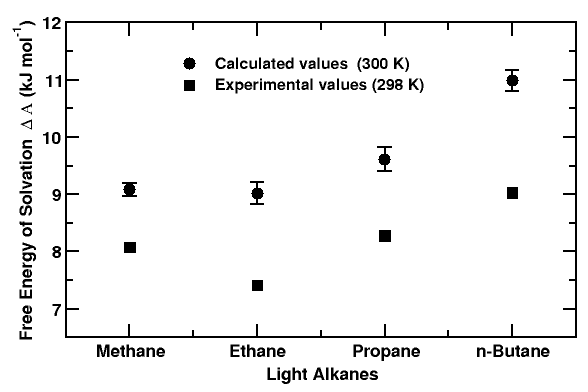
\includegraphics[scale=0.38]{Chapter4/comparison.png}
\caption[Solvation free energy of light alkanes in TIP3P water.] { Calculated values of solvation free energy of alkanes (methane, ethane, propane and n-butane) in TIP3P water at 300 K and the experimental values at 298 K.}
\label{alkanecompare}
\end{figure}
%%%%%%%%%%%%%%%%%%
 
 
 %%%%%%%%%%%%%%%%%%
 \begin{figure}[h!]
  \centering
 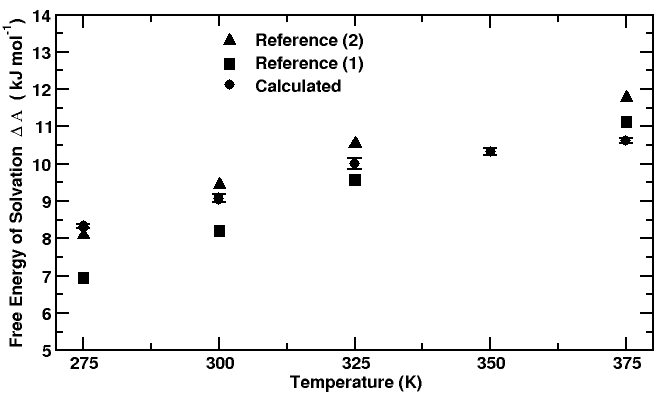
\includegraphics[scale=0.38]{Chapter4/Methane_compare.png}
  \caption[Comparison of calculated and literature values of free energy of solvation of methane in water at different temperatures. ]{ Comparison of calculated and literature values (Reference(1)~\citep{paschek2004temperature, fernandez2004aqueous}, Reference(2)~\citep{docherty2006potential} of solvation free energy of methane in water at different temperatures.}
  \label{methanecompare} 
  \end{figure}
  %%%%%%%%%%%%%%%%%%
  
  \begin{table}[H]
   \centering
   \caption[Solvation free energies of methane in water at different temperatures.] {Calculated and references (experimental and literature) values of  solvation free energies ($\mathrm{kJ mol^{-1}}$ ) of methane in water at different temperatures.}
    \label{methane_free}
  \resizebox {0.60\textwidth }{!}{%
  \begin{tabular}{ |c| c| c|  c|  c|    }
  \hline       
  {Molecule} & T (K)  &  Calculated &   Ref.(1)\citep{paschek2004temperature, fernandez2004aqueous}   &   Ref.(2)~\citep{docherty2006potential}  \\ \hline  
   & 275 &	  8.33 $\pm$ 0.05 & 6.95 &  8.09  \\ 
    & 300 &	  9.08 $\pm$ 0.12 & 8.21   &  9.45  \\
    Methane  &  325  & 10.01 $\pm$ 0.14  & 9.58  &  10.54 \\  
    & 350 &	  10.32 $\pm$ 0.09 & ---  &   ---  \\ 
    & 375 &	  10.63 $\pm$ 0.07 & 11.13 &   11.78 \\  
   \hline 
  \end{tabular}}
  \end{table}
  
  The comparison between the  calculated values with error bars of solvation free energy of alkane in water at 300 K and the corresponding experimental values at 298 K is shown in figure (\ref{alkanecompare}). Similarly, the comparison of calculated and literature values of   free energy of solvation of methane in water at different temperatures  in shown in figure (\ref{methanecompare})  and tabulated in table (\ref{methane_free}). The free energy of solvation of alkanes (methane, ethane, propane and n-butane) in methanol  as a fuction of temperature is plotted in figure (\ref{alkanemethanol})
  
   %%%%%%%%%%%%%%%%%%
   \begin{figure}[h!]
    \centering
      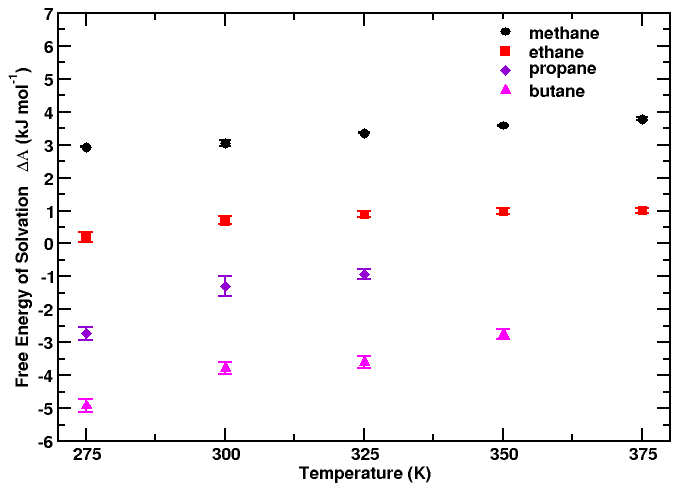
\includegraphics[scale=0.38]{Chapter4/alkane_methanol.png}
   \caption[Solvation free energy of alkane  in  methanol at different temperatures.]{Solvation free energy of alkane  in  methanol at different temperatures, from T = 275 K to T = 375 K.}
   \label{alkanemethanol}
   \end{figure}
 %%%%%%%%%%%%%%%%%%
 
 The solvation process is considered to consist of two steps, (i) the formation of a repulsive cavity of appropriate size, and (ii) the introduction of the solute into this cavity. The positive values of calculated  free energies of solvation ($\Delta A$) in  TIP3P water   for all of the alkanes (methane, ethane, propane and n-butane) indicate their low solubilities in water that means alkanes are hydrophobic in nature. The simulations also show, in
 accordance  with experiment, that $\Delta A$ decreases from methane to ethane, but then increases with increasing carbon number for longer up to butane at 300 K. This shows that the methyl group of alkane molecules have a preferential tendency to be dissolved in the vicinity of water molecules and that this tendency decreases with
 chain length. The increase in free energy of solvation with increase in temperature   describes  that the formation of repulsive cavity in water is perturbed by the thermal agitation of the water molecules. That means when temperature is incresed  we don't have new interactions that are strong enough to introduce some important change in enthalpy and change in Helmoltz free energy $A$  is mostly connected with entropy or reordering of hydrogen bonds. By placing alkane in water  we are perturbing the hydrogen bond  network so that water molecules need to reorganize themselves around the solvent in a particular way that makes possible for average number of bonds for one molecule to remain  constant. Since hydrogen bonds are directional this leads to a smaller configurational space for
 water  molecules  and change in entropy will be negative~\citep{Wu2008, abraham1988temperature}. Again , we have calculated free energy of solvation of alkanes in methanol at different temperatures. From table (\ref{freeenergy_table}) and figure (\ref{alkanemethanol}), free energy of solvation $\Delta A$  in methanol becomes more negative as the alkane chain increases. The positive values of solvation free energy of methane and ethane shows that they are insoluble in methanol but the negative values of it for propane and butane indicates they are soluble in the methanol. Methanol is  amphiphilic organic substance. There  is a competition between hybrophobic group (methyl-CH3) and a hydrophilic group (hydroxyl-OH). Amphiphilic nature makes methanol interesting solvent because alkanes should show greater solubility in it than in water. For methane and ethane the hydrophobic groups dominates over the hydrophilic group, on the other hand for propane and butane the reverse situation occurs.  
   

 



 